% ============================================================
% SDU Project Report Template
% ============================================================
\documentclass[12pt, a4paper]{report}

% --- Packages ---
\usepackage[utf8]{inputenc}
\usepackage[T1]{fontenc}
\usepackage[english]{babel}
\usepackage{geometry}
\usepackage{graphicx}
\usepackage{hyperref}
\usepackage{setspace}
\usepackage{titlesec}
\usepackage{tocloft}
\usepackage{fancyhdr}
\usepackage{lipsum}     % Remove in final report (used for placeholder text)
\usepackage{array}
\usepackage{booktabs}
\usepackage{float}
\usepackage{caption}
\usepackage{subcaption}
\usepackage{enumitem}
\usepackage{lmodern}
\usepackage{xcolor}
\usepackage{listings}   % For code listings if needed

% --- Page Geometry ---
\geometry{
    a4paper,
    top=2.5cm,
    bottom=2.5cm,
    left=3cm,
    right=2.5cm
}

% --- Line Spacing ---
\onehalfspacing

% --- Header / Footer ---
\pagestyle{fancy}
\fancyhf{}
\fancyhead[L]{\leftmark}
\fancyhead[R]{\thepage}
\renewcommand{\headrulewidth}{0.4pt}

% --- Hyperlink Setup ---
\hypersetup{
    colorlinks=true,
    linkcolor=black,
    urlcolor=blue,
    citecolor=black
}

% ============================================================
% FRONT PAGE
% ============================================================
\begin{document}

\begin{titlepage}
    \centering

    % SDU Logo — replace path with actual logo file
    
\includegraphics[width=0.8\textwidth]{Images/SDU-logo-sort.png}\\[2cm]

    {\Huge \textbf{Project Name}}\\[0.5cm]
    {\large Semester X, Year XXXX}\\[2cm]

    \begin{tabular}{ll}
        \textbf{Students:} & Student Name 1 \quad \texttt{stud1@student.sdu.dk} \\
                           & Student Name 2 \quad \texttt{stud2@student.sdu.dk} \\
                           & Student Name 3 \quad \texttt{stud3@student.sdu.dk} \\[0.5cm]
        \textbf{Supervisor:} & Supervisor Name \\[0.3cm]
        \textbf{Lecturers:} & Lecturer Name 1 \\
                            & Lecturer Name 2 \\
    \end{tabular}

    \vfill
    {\large University of Southern Denmark}\\
    {\large \today}
\end{titlepage}

% ============================================================
% FRONT MATTER (not counted in written page count)
% ============================================================

% --- Table of Contents ---
\pagenumbering{roman}
\tableofcontents
\newpage

% --- List of Figures ---
\listoffigures
\newpage

% --- List of Tables / Diagrams ---
\listoftables
\newpage

% --- Abstract ---
\chapter*{Abstract}

\addcontentsline{toc}{chapter}{Abstract}

% A short summary of the project, the report and what the reader
% will get from reading it.

\noindent
This report describes the semester project provided by Danfoss. 
The project is creating a heat production optimization interface for a district and applying agile and scrum methodologies.
The report will cover the development process, solutions, implementation and group collaboration.
The reader will gain insight into how the project was structured, how certain challenges were overcome, the planning process and the final product of the project.

\newpage
\pagenumbering{arabic}

% ============================================================
% CHAPTER 1 — INTRODUCTION
% ============================================================
\chapter{Introduction}
% An introductory chapter contextualising the project and the specific
% module or set of tasks worked on.


\section{Project Objectives and Requirements}

% Describe the project objectives and requirements. Include a brief outline
% of the methods and processes used.

The main objective of the project is to create an application for heat production optimization for a district heating utility,
optimizing heat production for the lowest cost, 
while allowing for two scenarios with different production assets, winter and summmer periods and enabling for maintenance periods.
The system must be separated into five modules: asset manager, source data manager, result data manager, optimizer and data visualization. 

The project has been divded into tasks for each sprint and distributed among all group memebers,
while having frequent ceremonies to ensure everyone keeps up with the workflow.


\section{Problem Statement}

% State the problem your project addresses. This should be a clear,
% concise formulation of the issue you set out to solve.

District heating utilities need to provide heat to all buildings in the districts heating network.
Providing heat to all buildings can become expensive and unsustainable, especially during winter periods where the heat demand is high.
An application can help manage the heating utilities by optimizing heat production for the lowest cost
and allowing for maintenance while simultaneously displaying the optimization results.

% ============================================================
% CHAPTER 2 — SCRUM IMPLEMENTATION
% ============================================================
\chapter{Scrum Implementation}
\section{Scrum selection}

For this project, our goal was to create a heat optimization desktop application for Danfoss that could read data sheets, calculate production costs, track emissions and optimize based on two scenarios. Although these requirements were to a great extent well-understood from the outset of the project, we had to navigate technical uncertainty and our limited experience delivering such requirements in teams. Hence, Scrum was our preferred choice, even though it was strictly mandated by the semester project course and expectations, it enabled us to deliver iteratively, reflect on our experience and limitations, and adapt as we progressed through.

\section{Sprints}

We split our project timeline into a setup phase(Sprint 0), followed by five development sprints. If a sprint is too short, like one week, you spend too much time in meetings planning and reviewing instead of actually writing code. If a sprint is too long, like a month, we procrastinate because the deadline feels too far away. We kept each sprint two weeks long and found that a two-week schedule was the perfect length for our group as it gave us enough time to actually design, code, and test a working part of the app, but it was short enough to keep everyone focused and accountable.

\section{Team organization and roles}

In the spirit of Agile principles, we made a conscious decision to rotate the Scrum role among team members and emphasize collaboration over strict hierarchical structures and predefined roles. For example, throughout the project, the role of the Scrum Master was assumed by two different members. Instead of locking one person into an unchangeable position for the entire semester, this rotation strategy distributed ownership across the group. The Scrum Master focused on maintaining our Jira board, tracking deadlines and organizing our examinations of the code. This approach ensured that the responsibility for managing team workflows was shared fairlyand kept our sprints moving forward efficiently.

For the Product Owner (PO) role, we decided to share its responsibilities, which enabled a shared sense of accountability for the product's features and quality. Because our student group consists of six colleagues who all interacted directly with stakeholders and supervisors, isolating a single individual as our source of requirements would have slowed down communication. Instead the feedback we received from Danfoss in the midterm evaluation was owned by all team members. For example, when requested to add a CO2 emissions tracking graph, the entire group collaborated to map out the required features. Every member took part in translating these expectations into clear backlog items.

We used a volunteering approach in our meetings for asigning of the taks, where everybody volunteered based on their interests, technical strengths, and to keep everything fair, which worked really well for us and helped divide our work evenly.

\section{Scrum ceremonies adoption}

We followed the main ideas for the four Scrum meetings (Planning, Daily Standups, Reviews, and Retrospectives) but adapted them to fit our schedules as students. Even though we all shared the same university schedule, of course everyone also had commitments outside of classes and other personal activities.

Our Sprint Planning meetings took place every Monday at the start of the sprint and usually lasted around an hour. In this sessions we reviewed our backlog (see Appendix \ref{app:product_backlog}) and agreed on what we wanted to get done next. We used story points as a simple way of estimating the effort needed to finish them, but we also relied on our own inutition of how difficult a task seemed and how much free time we had available during that sprint. Before a task could be added to the sprint board everyone needed to understand what was required and how it should be implemented.

The Daily Scrum was the ceremony that we adapted the most. In theory Scrum suggests a short daily meeting where everyone shares updates. But for us, meeting in person every day was not the best use of our time. What we did instead was that we held one dedicated in person meeting each week to discuss progress and if any issues appeared and needed attention but for the rest of the week we stayed in contact through a WhatsApp group chat. Everyone posted updates whenever they completed a task or maybe if they ran into a problem which allowed us to stay informed without needing to meet every day and offeres us more flexibility.

We also combined the Sprint Review and Sprint Retrospective into a single session that took place when the sprint ended. In the review we tested the latest version of the app together and checked if the features worked as expected. After that we discussed how the sprint had gone, what worked well and what could be improved in the next sprint.

\section{Jira for workflow management}

When we set up the project in Sprint 0 we considered both Trello and Jira~\cite{jira}. Even though Trello was quite easy to understand and had a simple layout we thought Jira seemed better suited for a software development project because it offered more ways to organize our tasks and track the progress. One more reason is that we preferred Jira's interface because it is a very feature rich tool and the benefit of using it was that it is very used in the industry so getting some experience with it felt reasonable for future projects, therefore it was an easy choice.

Our setup was very simple, we organized the board into six columns that replicated how the tasks actually moved through the project:

\begin{itemize}
    \item Backlog - all of the existing tasks we have written (a comprehensive record of these items is available in Appendix \ref{app:product_backlog})
    \item To Do - tasks we chose for this sprint but haven't been started yet
    \item In Progress - tasks that were worked on in that moment
    \item In Review - tasks that were completed and for which the team needed to review the code first
    \item Testing - tasks that were completed but needed some manual testing to see if they behave correctly
    \item Done - tasks that have been approved by everybody and merged into the main branch~\cite{git}
\end{itemize}

Tasks often moved quickly between the columns because we were in constant connection with the whatsapp group, but having the board available made it easy to see what still needed attention before the end of each sprint.


\section{Delineations from Scrum recommendations}

It is clear that our team did not follow Scrum exactly as it is described but we treated it as a guideline and made it fit the realities of a six person student project.

Such framework is designed for professional development teams that work full-time but our situation was quite different and for us trying to follow every Scrum rule would probably just have added unnecessary complications without much additional value.

Because of this we focused on the parts of Scrum that genuinely helped us work together, as we still planned our work in sprints, maintained a backlog, held regular meetings and reflected on our process, but we adapted the details to suit our needs. For example we used story points as a rough guide instead of relying on time estimates, communicated through WhatsApp instead of holding daily in person standups and combined some meetings to spend less time spent on managing our collaboration. We deemed this lightweight implementation sufficient for our project and well-aligned with our academic circumstances.

Overall we believe our approach was successful even if it was less formal than a classic Scrum implementation, because it was well suited to our circumstances and most importantly it helped us deliver a fully functional application that met all of the requirements provided by Danfoss.


% ============================================================
% CHAPTER 3 — SPRINTS
% ============================================================
\chapter{Sprints}
\section{Sprint 0}

 

\subsection*{Summary}

Sprint 0 was started on 15 February and was used as a preparation sprint to set up the entire project infrastructure, including the project repository in GitHub, the project management board in Jira for the SCRUM process, and communication channels as a WhatsApp group. The main goal was to establish the Scrum process and define the initial system structure before starting implementation in sprint 1. 

Also in this sprint, the team had its first meeting with the supervisor and distributed roles between members. A project backlog with user stories and tasks, epics, and assigned them to the team, and made the first UI concept.

\subsection*{Deliverables}

The main deliverable of Sprint 0 was the project backlog with user stories and tasks, epics, and they were assigned them to the team. Also, the project repository was created in GitHub, and the project management board in Jira for the SCRUM process. The team tasks on sprint 0 were:

\begin{itemize}

    \item Create a draft how the product should look like

    \item  Define three-layer architecture

    \item Define high-level UI structure

    \item Define UML class

    \item Jira board and initial Product Backlog
    
    \item GitHub repository

\end{itemize}

 

\subsection*{Sprint Planning}

During Sprint planning, the team chose to start work on setup tasks and workflow preparation,flow, and left coding for the next sprints. The main focus was on app architecture and Scrum process. 

Also, the team discussed what the project should look like. In the Jira workflow, it was decided to make epics for major project areas, so tasks and User Stories could be grouped more clearly and transparently. Also, distributed roles for the first demo presentation. Evidence of Sprint 0 Planning and Review can be found in Figure~\ref{fig:sprint0-planning-review}.



 

\subsection*{Sprint Review}

During the sprint review, the team presented the project backlog with User Stories and tasks, epics, and how tasks and user stories were assigned to team members. As well, the project repository was created in GitHub, the project management board in Jira for the SCRUM process, and communication lines as a WhatsApp group. The first UI concept of an application was demonstrated. 

The feedback from the Danfoss representative, teacher, and supervisor showed that the team needed to define project requirements more clearly, and the team should finish User-Stories and tasks for all sprints in Backlog.

Based on this feedback, the team decided to improve the backlog structure and use Jire more actively in the following sprints. Evidence of Sprint 0 Planning and Review can be found in Figure~\ref{fig:sprint0-planning-review}.

 

\subsection*{Sprint Retrospective}

What went well:

\begin{itemize}

 \item Basic project infrastructure was successfully created

 \item GitHub, Jira, and communication channels were set up

 \item The first Product Backlog and UI concept were prepared

\end{itemize}



What did not go well:

\begin{itemize}

 \item The project scope was still not fully clear
 
 \item The backlog was not detailed enough  
 
 \item The team was still learning how to document Scrum ceremonies properly

\end{itemize}



Improvement:

\begin{itemize}

 \item Improve meeting documentation and Scrum evidence

 \item Refine the Product Backlog in future sprints

 \item Assign tasks more clearly between team members

\end{itemize}

Sprint 0 Retrospective evidence can be found in Figure~\ref{fig:sprint0-retrospective}.

\subsection*{Reflections and Conflicts}

The main difficulty was the uncertainty about project expectations. The team didn’t have a clear view of how the application should work, and realized. As well, the team was not fully confident in the level of detail for Scrum documentation. This question was solved in a meeting with supervisor Alan and after the first demo feedback.

 

% --------------------------------

\section{Sprint 1}

 

\subsection*{Summary}

Sprint 1 started on 2 March and served as an architecture and requirements sprint. The main goal was to focus on defining the system  requirements and UML diagrams before starting implementation and development work in later sprints. 

During this sprint, the team focused on turning the initial idea and concept into a structured design. To complete this work, the group began creating a Figma UI prototype. First, an AI-generated Figma version of the app UI was created to explore possible design approaches. Afterward, a manually designed version was developed by a team member. Additionally, in Sprint 1, daily stand-up meetings were introduced to track progress and discuss task status, as part of implementing the Scrum process. In addition, the backlog was fully implemented, including all User Stories and tasks. The purpose of Sprint 1 was to start technical preparation for the next implementation.

 

\subsection*{Deliverables}

The main deliverables of Sprint 1 were preparing the technical setup, such as diagrams, functional/non-functional requirements, and a UI prototype for the following app development:

 \begin{itemize}
    \item Define functional and non-functional requirements
    \item Create Diagrams (UML, User case, Sequence, Component)
    \item Create a UI-Prototype in Figma

  \item Group Agreement document was created

\end{itemize}


\subsection*{Sprint Planning}

During Sprint Planning, the team discussed and defined the system requirements and architecture. Tasks were then the distributed between team members,such as defining functional and non-functional requirements, creating the all-important project diagrams, and developing a UI prototype. The selected backlog items were moved from the Product Backlog into the Sprint Backlog. Evidence of Sprint 1 Planning can be found in Figure~\ref{fig:sprint1-planning}.

 

\subsection*{Sprint Review}

During the Sprint Review, the group presented a Figma UI prototype, a document with high-level, functional, and non-functional requirements, a sequence diagram, a UML User case, and component diagrams.


The feedback from teachers and supervisors showed  that the team did good work, but they should improve their presentation skills and start working on technical aspects. The Sprint Review confirmed that the project was ready to move into implementation-focused sprints. Evidence of Sprint 1 Review can be found in Figure~\ref{fig:sprint1-review} and Figure~\ref{fig:sprint1-review-board}.

 

\subsection*{Sprint Retrospective}

What went well:

\begin{itemize}

 \item Functional and non-functional requirements were defined

 \item The first diagrams and UI prototype were created

 \item The team improved the Scrum workflow and daily stand-up meetings

\end{itemize}


What did not go well:

\begin{itemize}
    \item Some User Stories were unclear

    \item The backlog required more refinement and details

    \item The team needed better preparation for sprint presentations

\end{itemize}

Improvement:

\begin{itemize}
    \item Improve backlog refinement in Jira

    \item Prepare presentation materials earlier for future sprint reviews

\end{itemize}

Sprint 1 Retrospective evidence can be found in Figure~\ref{fig:sprint1-retrospective}.

\subsection*{Reflections and Conflicts}

During Sprint 1, there were no serious conflicts or problems. The issue of unclear User Stories was improved through backlog refinement in Jira. But in the next sprint presentation, the team decided to make better preparations for the Sprint 2 Demo to make it more professional.

 

% --------------------------------

\section{Sprint 2}

 

\subsection*{Summary}

Sprint 2 started on 16 March and was the start of program development. The main goal was to focus on Asset Manager, Source Data Manager, Optimizer base, and the first UI implementation for implementing scenario 1.

During this sprint, the team focused on using architectural plans to deliver working code. The first stage was to distribute the main system modules and responsibilities among team members. During the daily Scrum meetings, the team discussed component integration and verified that the modules matched the UML class design. One team member also participated in a representative meeting to discuss project progress and communication between groups. The team also demonstrated the first working results using Avalonia UI.

 

\subsection*{Deliverables}

The main deliverables of Sprint 2 were writing code for the main program components and implementing the draft UI:

  \begin{itemize}
    \item Source Data Manager implementation
    
    \item Optimizer logic for Scenario 1 was implemented
    
    \item  Implemented Asset Manager, ProductionUnit class, and UI for displaying production units

    \item Added support for two seasons in SourceDataManager

    \item Optimizer supports different scenarios based on the selected season

\end{itemize}



\subsection*{Sprint Planning}

During Sprint Planning, the team decided to start work on scenario 1. The team moved selected User Stories from the Product Backlog into the Sprint Backlog and identified a dependency chain between the modules: that AssetManager provides units, SourceDataManager provides heat demand/electricity prices, and Optimizer depends on SourceDataManager and AssetManager. And UI will show the current state. Each team member was responsible for a specific module or task. Evidence of Sprint 2 Planning can be found in Figure~\ref{fig:sprint2-planning}.

 

\subsection*{Sprint Review}

During the Sprint Review, the group presented the implemented Asset Manager and Source Data Manager, demonstrated the foundation of the optimizer logic and how the UI looks, and showed that the system structure was beginning to match the architecture defined in the UML class and component diagrams. Additionally, the maintenance functionality was not yet fully implemented. 

The feedback from teachers and the supervisor confirmed that the code and results are correct, but the group received a recommendation to improve the UI. The Sprint Review confirmed that the project was moving from design into implementation-focused development. Evidence of Sprint 2 Review can be found in Figure~\ref{fig:sprint2-review}.

 

\subsection*{Sprint Retrospective}

What went well:

\begin{itemize}

    \item The code runs well and was correctly pushed to GitHub

    \item Everybody kept up with the schedule 

\end{itemize}



What did not go well:

\begin{itemize}

    \item  Team members did not manage to implement the maintenance part for the project and moved it to the next sprint 

\end{itemize}



Improvement:

\begin{itemize}

    \item Team should make sure to take on only as much as they are sure they will be able to accomplish

    \item Additional tasks should only be added after the planned work is completed

\end{itemize}

{fig:sprint2-retrospective}.

\subsection*{Reflections and Conflicts}

The challenge was to distribute story points and prioritize tasks correctly, and some issues with GitHub branch management appeared in the first days of the sprint, but in the daily Scrum meetings, this problem was solved. 

 

% --------------------------------

\section{Sprint 3}

 

\subsection*{Summary}

Sprint 3 started on 27 March and focused on testing and finalizing Scenario 1. The main goal was to focus on creating unit tests for the code, finalizing the remaining features for Scenario 1, and starting to work on Scenario 2.

During this sprint, the team focused on finishing all code for scenario 1. One of the tasks was to complete all the UI so the program would be ready for the midterm evaluation. In addition to extensive unit testing for all main managers and optimizers, a major part of the unit tests included positive/negative/edge cases. Moreover, work started on Scenario 2 and on creating tests for it. In addition, after the LaTeX Workshop team began work on a Report Setup, Visual Studio Code was chosen as the main environment for writing the report in LaTeX.

 

\subsection*{Deliverables}

The important deliverables of Sprint 3 were writing tests for the main program components and implementing the full UI for Scenario 1:

\begin{itemize}
    \item  tests for GetProductionUnits()
    
    \item  tests for SourceDataManager

    \item  tests for RunScenario1()

    \item  tests for RunScenario2()

    \item  tests for GetUnitsByNetProductionCost()

    \item tests for CalculateNetProductionCost()

    \item  tests for CreateMaintenanceForBoiler()

    \item  Completed maintenance logic

    \item  UI for Scenario 1 becomes fully implemented and usable

    \item Completed report repository setup

    \item  Created presentation for midterm evaluation

\end{itemize}

 

\subsection*{Sprint Planning}

This sprint planning was conducted online. During sprint planning, it was decided to focus on unit testing existing methods and improving the UI for Scenario 1 at the end of the meeting. Each member was assigned a Jira testing story. After a recommendation from the supervisor, report-related tasks were added to the Jira backlog. The sprint scope was expanded after the planned tasks were completed earlier than expected. The sprint was more quality-focused than feature-focused. Evidence of Sprint 3 Planning can be found in Figure~\ref{fig:sprint3-planning}.

 

\subsection*{Sprint Review}

During the Midterm Evaluation, the group presented unit testing progress, a fully implemented UI, and the functionality of Scenario 1.

Feedback from teachers, the supervisor, and the Danfoss representative indicated that the graph visualization and UI presentation should be improved. All tasks planned during Sprint Planning were completed before the midterm evaluation. Evidence of Sprint 3 Review can be found in Figure~\ref{fig:sprint3-review}.

 

\subsection*{Sprint Retrospective}

What went well:

\begin{itemize}

    \item The code runs well

    \item Everybody kept up with the schedule 

    \item Unit tests increased confidence in the system

    \item The UI for Scenario 1 became fully usable

\end{itemize}



What did not go well:

\begin{itemize}

    \item  Minor time management issues
    
    \item  It was the team's first experience with the online Sprint Planning meetings
    
    \item  Scope changed during the sprint

\end{itemize}



Improvement:

\begin{itemize}

 \item Take only a realistic scope of work

 \item Improve time management to reduce delays

\end{itemize}

Sprint 3 Retrospective evidence can be found in Figure~\ref{fig:sprint3-retrospective}.

 

\subsection*{Reflections and Conflicts}

The presentation for the midterm evaluation was somewhat confusing. The team adjusted speaking roles to avoid repeating information during the presentation. The team also forgot to formally close the sprint on time. As a result, the sprint was completed after the midterm. Moreover, the team forgot to send the sprint 3 documentation to itslearning. To solve this problem, the group decided to send the documents for sprint 3 and sprint 4 together with the Sprint 4 submission.

 

% --------------------------------

\section{Sprint 4}

 

\subsection*{Summary}

Sprint 4 started on 20 April and focused on report writing and finalizing Scenario 2. The main goal was to finish the full program so that Scenarios 1 and 2 function correctly and to add more graphs to make the visualization clearer and easier to understand

During this sprint, the team focused on finalizing the remaining program functionality. One of the biggest improvements was adding Heat Demand graphs, CO2 emissions, and net production cost. In this sprint, the program became more prepared for the final demo, and the team continued preparing the program for the final demo.

\subsection*{Deliverables}

The important deliverables of Sprint 4 were the visualization part of the program: 

 \begin{itemize}

    \item  Report writing continued;
    
    \item  Heat Demand graph for Scenario 1

    \item  Heat Demand graph for Scenario 2

    \item  CO2 emissions graph

    \item  Net Production Cost graph

    \item UI restructuring based on midterm feedback

    \item  Tests for CreateMaintenanceForBoiler()

    \item  CO2 emissions integration into the optimizer

    \item  Result visualization improvements

\end{itemize}


 

\subsection*{Sprint Planning}

Sprint 4 planning started on 20 April, after the midterm, in an offline mode. During this sprint, the team distributed UI visualization tasks and checked the status of the report. Also, the midterm feedback was discussed, along with how to implement all programs with features in the sprint timeframe. Moreover, after the supervisor’s recommendation, the team added a Jira backlog task related to Avalonia unit testing. Evidence of Sprint 4 Planning can be found in Figure~\ref{fig:sprint4-planning}.

 

\subsection*{Sprint Review}

During the Sprint 4 demo, the group presented the results of their work, including new graphs. In addition, using the presentation techniques learned during the additional presentation skills session.

Feedback from teachers and the supervisor confirmed that the work was completed correctly, but the graph should be more colorized and user-friendly for workers, and the team received recommendations to add more unit tests and improve UI. Evidence of Sprint 4 Review can be found in Figure~\ref{fig:sprint4-review}.

 

\subsection*{Sprint Retrospective}

What went well:

\begin{itemize}

    \item The team successfully implemented the midterm feedback

    \item graphs were added

    \item report work continued

    \item UI improved

\end{itemize}



What did not go well:

\begin{itemize}

    \item  Minor time management issues due to the Math exam

    \item  Report writing and development overlapped during the sprint

\end{itemize}



Improvement:

\begin{itemize}

    \item Split work more equally

    \item Continue and finalize report writing

\end{itemize}

Sprint 4 Retrospective evidence can be found in Figure~\ref{fig:sprint4-retrospective}.
 

\subsection*{Reflections and Conflicts}

The main challenge of this sprint was a Math exam scheduled for the same time. Because of the overlapping exam period, the team tried to complete all tasks after the exam within a limited amount of time. The team had to balance project work, report writing, and exam preparation at the same time.

% --------------------------------

\section{Sprint 5}

 

\subsection*{Summary}

Sprint 5 started on 1 May and focused on finalizing the project and unit tests,completing reports, and updating diagrams. The main goal was to finish all parts of the project, from code and diagrams to report and meeting logs before presenting the final version of the project

During this sprint, the team focused on improving and polishing the UI of the program, for example, improving button visibility and UI interaction feedback, and finishing report chapters and receiving feedback on them. Moreover, checking and improving diagrams of the project to make it accurately matched the implemented code. Finally, receiving feedback from the supervisor on how to improve the visual part of the app.

\subsection*{Deliverables}

The main deliverables of Sprint 5 were the finalizing report and program: 

\begin{itemize}
    \item  all unit tests implemented
    
    \item report close to the final version

    \item  All managers and optimizer components worked correctly

    \item  graph functionality testing

    \item  manual testing

    \item final demo preparation

\end{itemize}


 

\subsection*{Sprint Planning}

Sprint 5 planning started on 4 May in an offline meeting. During this sprint, the team distributed tasks, making the UI clearer and more user-friendly. The team also decided to add additional unit tests for graphs in Scenario, and these tasks were added to the Sprint Backlog. Each team member was assigned responsibility for checking unit tests related to a specific manager or module and adding positive, negative, and edge cases where possible. Also, the team decided to prepare for the final demo and demonstrate how the program works in different conditions. Evidence of Sprint 5 Planning can be found in Figure~\ref{fig:sprint5-planning}.


 

\subsection*{Sprint Review}

During the final demo, the group presented the final version of the application to Danfoss representatives, teachers, and supervisors. In this presentation, the team demonstrated all tabs of the program and the flexibility of graphs.

Feedback from Danfoss representatives, teachers, and the supervisor confirmed that the programs work absolutely correctly, and the graphs looked good. The supervisor gave some various design improvements, such as bigger fonts in Asset Manager, clearer selected scenario/seasons, allowing multiple maintenance units, or warning if demand is not being used, and improving the Data tab as a button/page. Evidence of Sprint 5 Review can be found in Figure~\ref{fig:sprint5-review}.

 

\subsection*{Sprint Retrospective}

What went well:

\begin{itemize}

    \item All unit tests were implemented;

    \item Main branch was stabilized;

    \item Report writing continued successfully

    \item UI improved

\end{itemize}



What did not go well:

\begin{itemize}

    \item Report still unfinished

    \item Diagrams were outdated/missing until late

    \item Some test mismatches occurred after changes in the codebase

\end{itemize}



Improvement:

\begin{itemize}

    \item Focus on finishing the report

    \item Update diagrams

    \item Ensure tests are updated when code changes

\end{itemize}

Sprint 5 Retrospective evidence can be found in Figure~\ref{fig:sprint5-retrospective}.
 

\subsection*{Reflections and Conflicts}

There was an issue that the code needed to be updated at the last moment before the final demo, but this problem was quickly resolved, and the final demo was completed successfully. The final phase required balancing report writing, UI polishing, diagram corrections, and final testing at the same time.

% ============================================================
% CHAPTER 4 — SOLUTION (TECHNICAL ASPECT)
% ============================================================
\chapter{Solution (Technical Aspect)}
This chapter presents the important UML diagrams used in the project.
For each diagram: explain what it represents, explain which part of the
system it models, justify why it is relevant, and connect it to the
implemented solution. You must produce at least one of each UML diagram
type taught in class: Package, Class, Activity, and Sequence. Older
versions or less important diagrams can be referenced from the Appendix.

% --------------------------------
\section{Package Diagram}

Describe the organisation of the system into major modules or layers.
Explain what the diagram represents, which part of the system it models,
why it is relevant, and how it connects to the implemented solution.

\begin{figure}[H]
    \centering
    % \includegraphics[width=0.8\textwidth]{diagrams/package_diagram.png}
    \caption{Package Diagram}
    \label{fig:package-diagram}
\end{figure}

% --------------------------------
\section{Class Diagram}

Describe the main classes, attributes, methods, and relations. Explain
what the diagram represents, which part of the system it models, why it
is relevant, and how it connects to the implemented solution.

\begin{figure}[H]
    \centering
    % \includegraphics[width=0.9\textwidth]{diagrams/class_diagram.png}
    \caption{Class Diagram}
    \label{fig:class-diagram}
\end{figure}

% --------------------------------
\section{Activity Diagram}

Describe the logic of an important workflow or process. Explain what the
diagram represents, which part of the system it models, why it is
relevant, and how it connects to the implemented solution.

\begin{figure}[H]
    \centering
    % \includegraphics[width=0.75\textwidth]{diagrams/activity_diagram.png}
    \caption{Activity Diagram}
    \label{fig:activity-diagram}
\end{figure}

% --------------------------------
\section{Sequence Diagram}
Describe the interaction between objects or components for a key use
case. Explain what the diagram represents, which part of the system it
models, why it is relevant, and how it connects to the implemented
solution.

\begin{figure}[H]
    \centering
    % \includegraphics[width=0.85\textwidth]{diagrams/sequence_diagram.png}
    \caption{Sequence Diagram}
    \label{fig:sequence-diagram}
\end{figure}

% --------------------------------
\section{Overall Technical Architecture}

\subsection{High-Level Structure}
The application was built using the Model-View-ViewModel (MVVM) architectural pattern because it provides a nice structure for organizing our code and makes it easy to separate the user interface from the actual code logic since our project involved both a visual dashboard and an optimization system, which helped keep the codebase manageable as it got bigger.

\subsection{The Technology Stack}
To build the application we used C\# making use of the object-oriented structure to represent the different heat production units and optimization rules in our system.

For the user interface we chose Avalonia UI because it fits the MVVM design pattern perfectly and to create the graphs we used the LiveCharts2 library since a large part of the project involved presenting optimization results in a way that was easy for users to understand.

For data storage since the project was based on two static CSV files, WinterSourceDataSheet.csv and SummerSourceDataSheet.csv, we read them directly into memory and because the data was fixed and did not need to be edited by users, a database would have added extra complexity without any benefits.

\subsection{Separation of Concerns}

To make the project easier to understand and work on as a team we devided the app into four layers: the View Layer, the ViewModel Layer, the Domain Layer, and the Data Access Layer

Only the appearance of the program is controlled by the view layer as it contains files that specify UI elements including grids, buttons, sliders, date pickers, and more, like AssetView.axaml and ResultView.axaml.

Data binding connects the UI to the ViewModels, like when a user clicks a butto, the ViewModel collects the input data, sends it to the backend logic and after receiving the results it updates the UI automatically.

The domain layer doesn't know about the user interface and focuses just on calculations, in short being the logic of the app.

The Data Layer is loads the data into the system by reading the CSV files and converting them into usable structures like lists.

\subsection{Rationale for the Chosen Structure}

Using this separated structure helped us reduce the dependencies between parts of the code and it also helped with working on different parts of the app at the same time while not running into problems and merge conflicts.

For the data, again instead of introducing a database we simply loaded our fixed CSV files as lists when the application starts and it made things much more simple for the current scope of this project since there was no real need for a more complex solution.


% ============================================================
% CHAPTER 5 — IMPLEMENTATION AND TECHNICAL REALIZATION
% ============================================================
\chapter{Implementation and Technical Realization}


% --------------------------------
\section{Frontend Implementation}

The frontend was implemented in the UI layer using the Avalonia UI frameworks together with the MVVM (Model--View--ViewModel) architecture.  
The implementation focused on separating the UI layer from the Domain layer and Data layer in order to improve scalability and code readability. 

\subsection{Frontend Architecture}

The frontend was structured into multiple ViewModels and Views:


\begin{itemize}
    \item MainViewModel.cs (MainWindow.axaml)
    \item AssetViewModel.cs (AssetView.axaml)
    \item DashboardViewModel.cs (DashboardView.axaml)
    \item ResultViewModel.cs (ResultView.axaml)
    \item UnitConfigViewModel.cs
    \item ChartBuilder.cs
\end{itemize}



\subsection{Main Navigation and View Handling}

The MainViewModel was used as the center for navigation between different pages of the application. 
The ViewModel has a CurrentViewModel property which determined which page was displayed in the main content area. When the user selected a different tab in the navigation menu the Navigate() method updated the active ViewModel.
The tabs were stored using the currently selected tab through the SelectedTab property. 


\subsection{Asset Management Interface}


The Asset Management page was implemented to allow users to:

\begin{itemize}
    \item See details of production units
    \item Change between scenaios 
    \item Put units into maintenance
\end{itemize}
The page logic was implemented inside the AssetViewModel.  
Each production unit had its own separate UnitConfigViewModel which stored unit specific information such as maintenance and its duration.

\noindent \newline Two independent configuration were implemented:

\begin{itemize}
    \item \_scenario1Configs
    \item \_scenario2Configs
\end{itemize}
This was added so that changes made in one scenario did not affect the other scenario.  


\noindent \newline A maintenance check was implemented through the RefreshMaintenanceWarning() method.
Which calculated whether selected maintenance schedules could cause less heat compared to heat demand.
If maintenance risked creating less heat then needed a warning message was displayed to the user.  


\subsection{Data Interface}

The Data page provided users with a overview of system information and operational data. The purpose of this page was to give quick access to key system information before running the optimization.



\subsection{Result Visualization Interface}

The Result page is used to visualize the optimization output.
The page logic was implemented in the ResultViewModel while the graph generation was separated into the ChartBuilder class.

\noindent \newline The interface included:

\begin{itemize}
    \item Scenario selection buttons
    \item Winter/Summer selection buttons
    \item Graphs for the optimization
    \item Graph legends
    \item Time labels
\end{itemize}
Implemented graphs:

\begin{itemize}
    \item Heat production
    \item Heat demand
    \item CO$_2$ emissions
    \item Net production cost
    \item Electricity price (For Scenario 2)
\end{itemize} 
The heat production graph used stacked area charts to clearly tell apart production contributions from different units.  
To improve readability individual units were assigned colors and all graphs shared axis configuration methods.  
The graphs dynamically updated whenever the user changed scenarios or season selection.





\subsection{Communication Between Frontend and Backend}

The frontend communicated with backend through the ViewModels. The UI itself did not perform the optimization instead it sent information the user selected to the backend.

\noindent \newline When the user navigated to the Result page, the MainViewModel collected:

\begin{itemize}
    \item Selected scenario
    \item Selected season
    \item Selected production units
    \item Maintenance configurations
\end{itemize}

\noindent \newline These values were then passed into the ResultViewModel constructor:

\begin{verbatim}
CurrentViewModel = new ResultViewModel(
    _optimizer,
    AssetPage,
    scenario,
    isSummer,
    selectedUnits
);
\end{verbatim}

\noindent \newline The ResultViewModel then called the backend optimization methods:

\begin{itemize}
    \item RunScenario1()
    \item RunScenario2()
\end{itemize}



% --------------------------------
\section{Backend Implementation}

The backend was implemented into the Domain layer of the 3-layer architecture. The backend was responsible for handling optimization logic, maintenance scheduling, production unit management, and processing of operational data used by the UI layer.

\noindent \newline The backend consisted of the following classes:

\begin{itemize}
    \item Optimizer.cs
    \item ProductionUnit.cs
    \item MaintenanceCalculation.cs
    \item MaintenancePeriod.cs
    \item OptimizationResult.cs
    \item ResultFormatter.cs
\end{itemize}

\subsection{Backend Architecture}


\subsubsection{Optimizer Class}

The Optimizer class was used for running optimization scenarios and processing data.

\noindent \newline Its responsibilities included:

\begin{itemize}
    \item Loading seasonal data
    \item Calculating production costs
    \item Running optimization scenarios
    \item Generating optimization results
\end{itemize}
The optimizer received data from the Data layer through a dependency injection:

\begin{verbatim}
public Optimizer(ISourceDataManager sourceDataManager,
                 IAssetManager assetManager)
\end{verbatim}
The optimizer maintained separate dictionaries for seasonal datasets:

\begin{itemize}
    \item Summer
    \item Winter
\end{itemize}
Each dataset contained hourly operational data:

\begin{itemize}
    \item Heat demand
    \item Electricity prices
\end{itemize}

\subsubsection{ProductionUnit Class}

The ProductionUnit class represented individual heat production units.

\noindent \newline Each production unit contained:

\begin{itemize}
    \item Maximum heat production capacity
    \item Electricity generation
    \item Production costs
    \item Energy consumption
    \item CO$_2$ emissions
\end{itemize}
Availability checks were implemented using the IsAvailable() method:

\begin{verbatim}
public bool IsAvailable(DateTime time)
\end{verbatim}
This method made sure that units under maintenance were excluded form the optimization.

\subsubsection{MaintenanceCalculation Class}

\hbox{The MaintenanceCalculation class was used for scheduling maintenance for production units.}

The class created maintenance periods based on the users choices.

\noindent \newline The scheduling logic:

\begin{itemize}
    \item Located the selected production unit
    \item Created a maintenance period
    \item Assigned the maintenance interval to the unit
\end{itemize}


\subsubsection{ResultFormatter Class}

The ResultFormatter class was used for generating optimization reports.

\noindent \newline The implementation formatted optimization results into summaries that included:

\begin{itemize}
    \item Selected optimization scenario
    \item Seasonal configuration
    \item Maintenance schedules
    \item Hourly production schedules
\end{itemize}



\subsection{Business Logic Implementation}

The backend implemented two primary optimization scenarios.

\subsubsection{Scenario 1 -- Production Cost Optimization}

Scenario 1 optimized heat production by production cost.

\noindent \newline Optimization logic:

\begin{enumerate}
    \item Retrieved current heat demand
    \item Filtered available production units
    \item Sorted units by production cost
    \item Allocated heat production sequentially
    \item Continued until demand was satisfied
\end{enumerate}

\subsubsection{Scenario 2 -- Net Production Cost Optimization}

Scenario 2 extended the optimization logic by including electricity prices.

\noindent \newline The net production costs are calculated using:

\begin{equation}
\mathrm{Net\ Production\ Cost} =
\mathrm{Production\ Cost} -
\left(
\frac{\mathrm{Electricity\ MW}}
{\mathrm{Maximum\ Heat\ MW}}
\times
\mathrm{Electricity\ Price}
\right)
\end{equation}
This allowed the units that generated value through electricity to be prioritized. The unit rankings were updated every hour using the current electricity prices.

\subsection{Exception handling}

Exception handling was implemented to make sure the optimization can run.

\noindent \newline Implemented Exceptions:

\begin{itemize}
    \item Production unit capacity
    \item Dose the source data exist for a given time
\end{itemize}
If the production unit did not have MaxHeatMW an exception was thrown:

\begin{verbatim}
if (unit.MaxHeatMW <= 0)
{
    throw new ArgumentException(...);
}
\end{verbatim}


\subsection{Communication with the Data Layer}

The backend communicated with the Data layer through interfaces:

\begin{itemize}
    \item ISourceDataManager
    \item IAssetManager
\end{itemize}
These interfaces provided access to:

\begin{itemize}
    \item Seasonal operational datasets
    \item Production unit information
\end{itemize}
The actual loading of data was in the Data layer. 
This allowed the optimization logic to remain independent from data layer.


% --------------------------------
\section{Data Management}

The data management was implemented into the Data layer of the 3-layer architecture. It was used for managing operational data, production unit configurations and communication between the backend and external data.


\noindent \newline The Data layer was split into three primary components:

\begin{itemize}
    \item Asset Manager
    \item Source Data Manager
    \item Result Data Manager
\end{itemize}


\subsection{Data Layer Structure}

The Data layer consisted of the following main classes and interfaces:

\begin{itemize}
    \item AssetManager.cs
    \item IAssetManager.cs
    \item SourceDataManager.cs
    \item ISourceDataManager.cs
    \item ResultDataManager.cs
    \item IResultDataManager.cs
    \item DataPoint.cs
\end{itemize}
The layer also included external CSV files:

\begin{itemize}
    \item SummerSourceDataSheet.csv
    \item WinterSourceDataSheet.csv
\end{itemize}


\subsection{Asset Manager}

The AssetManager class was used for implementation of production unit information.
It also managed a list of ProductionUnit objects.

\noindent \newline Each production unit contained:

\begin{itemize}
    \item Unit name
    \item Maximum heat production
    \item Electricity production
    \item Energy consumption
    \item Production cost
    \item CO$_2$ emissions
    \item Image path
\end{itemize}
An example production unit implementation:

\begin{verbatim}
new ProductionUnit
{
    Name = "GB1",
    MaxHeatMW = 3.0,
    ProductionCost = 510,
    CO2Emissions = 132
}
\end{verbatim}
The AssetManager provided access to all production uinits through:

\begin{verbatim}
public List<ProductionUnit> GetProductionUnits()
\end{verbatim}


\subsection{Source Data Manager}

The Source Data Manager was used for loading and processing of operational data from CSV files.

\noindent \newline The SourceDataManager class loaded two datasets:

\begin{itemize}
    \item Summer operational data
    \item Winter operational data
\end{itemize}
The datasets were stored  as dictionaries:

\begin{verbatim}
Dictionary<DateTime, DataPoint>
\end{verbatim}
Each timestamp was attached to a DataPoint object containing:

\begin{itemize}
    \item Heat demand
    \item Electricity price
\end{itemize}
The DataPoint model was implemented as:

\begin{verbatim}
public class DataPoint
{
    public double HeatDemand { get; set; }
    public double ElectricityPrice { get; set; }
}
\end{verbatim}


\subsection{Result Data Manager}

The Result Data Manager class was used for storing optimization results. 

\noindent \newline Stored data for each hour in the optimization:

\begin{itemize}
    \item Scenario number
    \item Seasonal configuration
    \item Time
    \item Production unit name
    \item Heat production
    \item CO$_2$ emissions
\end{itemize}


\subsection{Exception handling}

Exception handling was implemented to make sure data can be read.

\noindent \newline Implemented exceptions:

\begin{itemize}
    \item Dose the CSV file exist 
\end{itemize}
If the file could not be found an exception was thrown:

\begin{verbatim}
throw new FileNotFoundException(...)
\end{verbatim}


\subsection{Communication with the Backend}

The Data layer communicated with the backend through a dependency injection.

\noindent \newline This allowed the backend to access:

\begin{itemize}
    \item Seasonal operational datasets
    \item Production units
    \item Structured optimization results
\end{itemize}






% ============================================================
% CHAPTER 6 — DISCUSSION & REFLECTION
% ============================================================
\chapter{Discussion \& Reflection}
% --------------------------------
\section{Scrum}

The first practice implemented was deciding who the Scrum Master will be, which proved to be a valuable decision, as he helped the team follow the Scrum framework, removed impediments, protected the process and coached the team. Appointing this role made the process of development easier, as the chaos was reduced, the structure of the ceremonies was followed and we were held accountable during the sprint. 

The ceremonies we adopted felt like a formality at first, but they quickly became useful for better code quality as well as better accountability. We always did the Sprint Planning on the first day of the Sprint, helping us distribute work evenly and create realistic goals, however the first times we underestimated or overestimated the effort required for tasks. The weekly standup with our supervisor, where everyone showed their progress, we fixed small tweaks, got feedback and continued the development process improved our code quality and direction. The Sprint Review where we inspected the increment and adapted the Product Backlog as well as the Sprint Retrospective where we created improvement actions and reflected on the Sprint, were done on the last day of the Sprint and made our sprint noticeably smoother by assigning better amounts of work tasks  and understanding the Scrum framework better.

Scrum artifacts like the Product Backlog where we had an ordered list of everything that might be needed in the product and the Sprint Backlog which were the tasks for the Sprint and using the Increment to meet the Definition of Done, helped us in knowing what tasks we have to develop, and what individual sprint was focusing on, which helped with better organizing and meeting deadlines accordingly.  

Other Scrum Practices we used were that we only had a single objective for each sprint, without sudden changes that could endanger the sprint goal, keeping transparency so that artifacts were visible and understandable to everyone, as well as regular inspection paired with adaptation. 

Some supporting practices we also used were using Story Points for User Stories for estimation, refining the Backlog and using Task Boards with the Kanban-style visualization inside the Sprint.

Overall, implementing Scrum taught us how important rhythm and discipline is in the development of software products, ceremonies that felt resistant, made us adapt and reflect better. The lesson we learned is that the framework is not about following rituals, but adapting a mindset of improving continuously, keeping transparency and maintaining collective ownership of the product.




% --------------------------------
\section{Requirements Engineering}

Requirements Engineering helped us during the Sprint Planning to plan and execute the work as well as to better understand the concept of the project~\cite{sommerville}. The practices and techniques made us discover, define, analyze, manage and validate user requirements to improve the efficiency and clarity of what we must do. This was a crucial part, because to fulfill the business needs of a product, the software team needs to understand the description of the service, functional and non-functional requirements to deliver the most optimal solution. 

Identifying the functional requirements benefited us by understanding system behaviors and what should it do, while the non-functional requirements informed us about the constraints we have on the system’s functionality, services and design. The process of identifying them started with the business objectives and high-level business requirements.

Following the right structure of defining everything needed and then starting to develop improved efficiency, as we knew exactly what do to, in what order, and how to implement them. Only after the requirements elicitation, analysis and specification, requirements documentation and requirements validation we started to work on the design and development of the Heat Optimization application. 

Another useful requirement engineering technique we used was creating the User Case Diagram, which helped us understand who are going to be the users of the app, and what cases each one will have to accomplish. 

Although the practices from requirements engineering bring better traceability and a rigid structure, they also added inconvenience to our inexperienced team. The ownership and continuous refinement of our Product Backlog and creating the documentation required extra effort and time, slowing down our overall development process. 

In this project, all requirements engineering techniques were useful and provided unique understanding for the goal we have to achieve, and we definitely consider to use them in future projects, in order to plan the development process and understand the nuances of the applications we have to build, but optimizing the mistakes we did so the process becomes smoother.



% --------------------------------
\section{Code Refactoring}

Code refactoring helped a lot in terms of improving the project’s code quality, as during development where multiple team members have different coding backgrounds, the code written did not always meet the cleanest standards. While updating the diagrams we noticed that some classes had too much functionality, which is bad for future scaling and performance optimizing. 

Refactoring also made sure that we applied Software Design Principles and learned how to use them in real coding situations, amplifying our knowledge over clean code principles. The main fixes we did during our code refactoring were, remaking repeated code into reusable functions and simplifying the code while maintaining the application functionality.

Some examples of that were making a single method for loading the graphs and calling it as many times as needed with different arguments, remaking the ResultViewModel class as it was handling too much functionality by splitting some parts into different files(moving
chart creation out of ResultViewModel and extracting UnitConfigViewModel in its own file), and removing the Optizimer singleton and creating an instance in App.axaml.cs.


% --------------------------------
\section{Code Review}

Code reviews played an important role in our understanding of the project and how the app works. When somebody was uploading some code, we were reviewing it with all the members so everyone would comprehend the logic and the syntax of the changes. 

The review sessions created the environment to clarify complex parts of code, suggesting better solutions and ideas for implementation and even catching issues early that would have costed us more time later in the project. In multiple cases, code reviews helped us solve conflicting code when more members were working on the same feature or class.

On the other hand, we also met some challenges during the sessions. Code reviews were time-consuming and there were cases where it was making the development process longer than we expected, when a feature needed multiple fixes or some ideas were conflicting in the search of finding the best approach. As a team with different coding backgrounds, aggreging on a coding style and architecture decisions were making us spend more time than we anticipated.
	
Even though we experienced the drawbacks of conflicts in code and our ways of thinking combined with more time spent as initially planned, the benefits of it made us understand how important the sessions were in the long run. The collaboration of the reviews improved the code base as well as understanding the system on a deeper level. In future situations, we also plan to use them, however implanting lighter review processes in order to reduce the time spent while benefiting from the advantages of sessions



% --------------------------------
\section{Testing}

In our product, we used multiple ways of testing which helped with the quality of it, by making sure all the boilers work as intended, graphs show the correct data output and the optimizer calculates the most optimal outcome. Starting with the Unit Tests ~\cite{xunit}~\cite{testsdk}, where we checked if the methods and functions for each class work as intended, by isolating them in separate test files. We managed to implement tests for all modules, graphs for both scenarios and crucial parts of the optimizer to make sure everything builds correctly. Functional testing was also used to check if each button works as intended, if we can choose the maintenance period for certain number of hours and the day, switching between tabs, as well as switching between scenarios and seasons. Finally, end to end testing assured us that the entire flow and actions of the app work and if the system can be delivered as planned.
	
There is a slight disadvantage with testing as it takes a generous amount of time implementing and making sure everything runs smoothly, however the benefits outweigh the drawbacks as having a system that is fully tested with code as well as manually guarantees a better product overall.

In future projects, we intend to integrate testing, as the software systems become more complex, the likelihood of more defects increases. Therefore, testing that each feature functions as planned becomes essential in order to maintain the reliability of the overall system. Without strict testing, multiple undetected issues can impact the performance of the application, leading to system failure and maintenance costs increase. This experience helped us to understand that the time invested in testing is worth to deliver high-quality and more stable software systems.  


% --------------------------------
\section{Overall Group Reflection}

\begin{table}[H]
    \centering
    \small
    \renewcommand{\arraystretch}{1.2}
    \caption{Requirement fulfillment comparison}
    \label{tab:requirements-comparison}
    \begin{tabular}{p{0.17\textwidth} p{0.28\textwidth} p{0.12\textwidth} p{0.33\textwidth}}
        \toprule
        \textbf{Requirement Category} & \textbf{Specific Requirement} & \textbf{Status} & \textbf{Comments / Changes Made} \\
        \midrule
        Modules & Implement all 5: AM, SDM, RDM, OPT, DV & Fully Met & All modules completed and integrated. \\
        Scenarios & Scenario 1 (3 gas boilers + 1 oil boiler) + Scenario 2 (2 gas boilers + gas motor + electric boiler) & Fully Met & Both scenarios implemented with correct unit behaviors. \\
        Time Periods & Winter \& Summer (14-day periods, 1-hour resolution) & Fully Met & Both periods loaded and optimized. \\
        Maintenance & Obligatory maintenance (30--60 hours) for at least one unit per scenario/period & Fully Met & Configurable via Asset Manager; enforced in Optimizer. \\
        Optimization Logic & Secure heat demand at all times; minimize net production costs (incl.\ electricity market) & Fully Met & Net production cost calculation implemented; priority-based scheduling. \\
        Data Handling & Use provided data (unit configs, heat demand, electricity prices) & Fully Met & Loaded from Danfoss files (Excel/CSV). \\
        Data Storage & AM: local files; SDM: CSV; RDM: CSV & Partially Met & Used only CSV for structure/readability, did not include JSON or other Databases. \\
        Data Visualization (DV) & Show grid, units, demand, production, electricity, costs, net costs, etc. & Fully Met & Interactive charts and diagrams implemented. \\
        Project Process & Architecture definition, domain/DTO objects, interfaces, subsystem + integration tests & Mostly Met & Full architecture and interfaces done; comprehensive unit tests; integration test covered main flows (some edge cases limited due to time). \\
        Additional Exercises & Database, API, unit activation from UI, Energinet API, etc. & Not Done & Did not implement any complex Databases or APIs. \\
        \bottomrule
    \end{tabular}
\end{table}

\begin{itemize}
    \item \textbf{Whether the product solves the stated issue.}
    \par\hspace*{1.5em}The stated issue was that HeatItOn always planned heat production schedules manually, which was difficult when ensuring continuous supply while minimizing production costs, maximizing profit, and handling fluctuating electricity prices and maintenance periods for boilers.
    \par\hspace*{1.5em}We addressed this issue with our application. Scenario 1 and Scenario 2 correctly prioritize cheaper units and use expensive units mainly during peak hours through net production cost logic in the optimizer. The solution meets heat demand while respecting maintenance periods, and the results are clearly visualized in the Results tab.


    \item \textbf{Whether the product leads to unforeseen problems that would be addressed with future development.}
    \par\hspace*{1.5em}Our optimizer uses a priority-based (greedy) scheduling algorithm based on net production costs. It currently works well for the two scenarios, but it can produce sub-optimal results in more complex situations. With strongly fluctuating electricity prices, a greedy approach may miss more profitable long-term combinations.
    \par\hspace*{1.5em}For the current 14-day periods, performance is solid. However, scaling to longer periods (for example one year) or multiple heating grids may introduce performance bottlenecks. In parallel, the data visualization module could become cluttered and less readable with larger datasets.
    \par\hspace*{1.5em}Maintenance periods are also limited in the current version. In a real-world scenario, maintenance rescheduling may be more dynamic, and the current structure would need to be extended.


    \item \textbf{Possible future development in terms of features, scalability, or other important factors.}
    \par\hspace*{1.5em}A strong technical improvement would be replacing the greedy algorithm with a Mixed-Integer Linear Programming solver to handle more complex constraints. Another key feature would be an API client for real-time electricity prices from a Danish source instead of relying only on static CSV data.
    \par\hspace*{1.5em}A scenario comparison tool would add value by allowing users to evaluate multiple configurations side by side. Data storage could also be upgraded from CSV to a relational database such as PostgreSQL to improve consistency, querying, and historical tracking.
    \par\hspace*{1.5em}From an operations perspective, an alarm and notification system could warn operators when demand cannot be met or when costs exceed budget thresholds. Additional improvements include PDF reporting with key indicators, deploying the app instead of running it only locally, and adding user-role management plus a mobile dashboard for practical professional use.

\end{itemize}


% ============================================================
% CHAPTER 7 — CONCLUSION
% ============================================================
\chapter{Conclusion}
% This chapter directly answers your project requirement. Structure it as
% follows:

%\begin{itemize}
%    \item Briefly summarise the key findings.
%    \item Provide a clear and final answer to the problem statement.
%    \item Highlight any objectives that were not fully achieved.
%    \item Suggest possible directions for future work.
%\end{itemize}

The project successfully achieved its goal of creating an application for district heat production optimization.
The system is fully dynamic and allows for heat optimization for the lowest cost, while enabling maintenance periods and different scenarios with different production assets, and different periods with varying heat demand. 

Everyone in the group equally contributed to the project and all of the objectives were achieved, however, not all of the non-required additional excercises were completed.

Due to scheduling and time constraints and mismanagement we were not able to complete everything as fast as we excpected to.

Future work would include better time management and more preparation for presentations and ceremonies to allow for better communication and improving the overall workflow.


% ============================================================
% REFERENCES (not counted in written page count)
% ============================================================
\chapter*{References}
\renewcommand{\bibname}{References}
\begin{thebibliography}{99}
\addcontentsline{toc}{chapter}{References}


\bibitem{avalonia} Avalonia UI, \emph{Avalonia Documentation (v11)}. [Online]. Available: \url{https://v11.docs.avaloniaui.net/}
\bibitem{avaloniamvvm} Avalonia UI, \emph{The MVVM Pattern}. [Online]. Available: \url{https://docs.avaloniaui.net/docs/concepts/the-mvvm-pattern/}
\bibitem{mvvmtoolkit} Microsoft, \emph{CommunityToolkit.Mvvm (MVVM Toolkit)}. [Online]. Available: \url{https://learn.microsoft.com/en-us/dotnet/communitytoolkit/mvvm/}
\bibitem{livecharts} B. Rodriguez, \emph{LiveCharts2}. [Online]. Available: \url{https://livecharts.dev/}
\bibitem{skiasharp} Microsoft, \emph{SkiaSharp}. [Online]. Available: \url{https://github.com/mono/SkiaSharp}
\bibitem{xunit} \emph{xUnit.net Documentation}. [Online]. Available: \url{https://xunit.net/}
\bibitem{testsdk} Microsoft, \emph{Unit testing in .NET}. [Online]. Available: \url{https://learn.microsoft.com/en-us/dotnet/core/testing/unit-testing-with-dotnet-test}
\bibitem{nuget} Microsoft, \emph{NuGet documentation}. [Online]. Available: \url{https://learn.microsoft.com/en-us/nuget/}
\bibitem{git} \emph{Git Documentation}. [Online]. Available: \url{https://git-scm.com/doc}
\bibitem{github} GitHub, \emph{GitHub Documentation}. [Online]. Available: \url{https://docs.github.com/}
\bibitem{jira} Atlassian, \emph{Jira}. [Online]. Available: \url{https://www.atlassian.com/software/jira}
\bibitem{sommerville} I. Sommerville, \emph{Software Engineering}, 10th ed. Harlow, U.K.: Pearson Education, 2016. [Book].

\end{thebibliography}


% ============================================================
% AI USAGE (not counted in written page count)
% ============================================================
\chapter*{AI Usage}
\addcontentsline{toc}{chapter}{AI Usage}



% \begin{itemize}
%    \item Which AI tools were used (e.g.\ ChatGPT, Copilot).
%    \item How the tools were used (e.g.\ brainstorming, improving
%          language, summarising information).
%    \item Which parts of the project were influenced by AI, if any.
%    \item How the AI-generated content was reviewed or modified by
%          the student.
% \end{itemize}

\noindent
During the course of the project, AI tools such as ChatGPT and Copilot were utilized,
primarily for brainstorming or finding suggestions in given situations, 
addittionally, AI tools were used for early prototyping and/or placeholder solutions that would later be replaced by manual overhauls.

Any AI-generated ideas that were considered were reviewed and evaluated in a group discussion, and expanded upon thusly.
AI-generated code, such as early prototypes, templates, examples, or placeholders were manually overhauled into more robust solutions.
Additionally, any other AI-generated content that was used during the course of the project was either discarded or manually overhauled to match the project's standards.


% ============================================================
% APPENDIX (not counted in written page count)
% ============================================================
\appendix

\chapter{Team Contributions}
Table of precise contributions of each team member for both the report
and the development part.

\begin{table}[H]
    \centering
    \begin{tabular}{lp{5cm}p{5cm}}
        \toprule
        \textbf{Student} & \textbf{Report Contributions} &
        \textbf{Development Contributions} \\
        \midrule
        Student 1 & & \\
        Student 2 & & \\
        Student 3 & & \\
        \bottomrule
    \end{tabular}
    \caption{Team Contribution Overview}
    \label{tab:contributions}
\end{table}

\chapter{Meeting Logs}

Include all meeting logs here: Scrum planning, stand-up meetings, Scrum
review, and retrospective logs that were not included in the main body.

\chapter{Contracts}

\section*{Supervisor Contract}
Insert or attach the contract with the supervisor.

\section*{Team Contract}
Insert or attach the contract with the team members.

\chapter{Code Authorship and Review}

Information about who is the author and reviewer for each part of the
code, e.g.\ classes and components.

\chapter{Other Supporting Documentation}

This appendix contains Scrum evidence materials from Jira and Confluence, including Sprint Planning, Sprint Review, and Sprint Retrospective screenshots.

%========================================================
\section{Sprint 0}
\label{app:sprint0}

\subsection*{Sprint Planning and Review}

\begin{figure}[H]
    \centering
    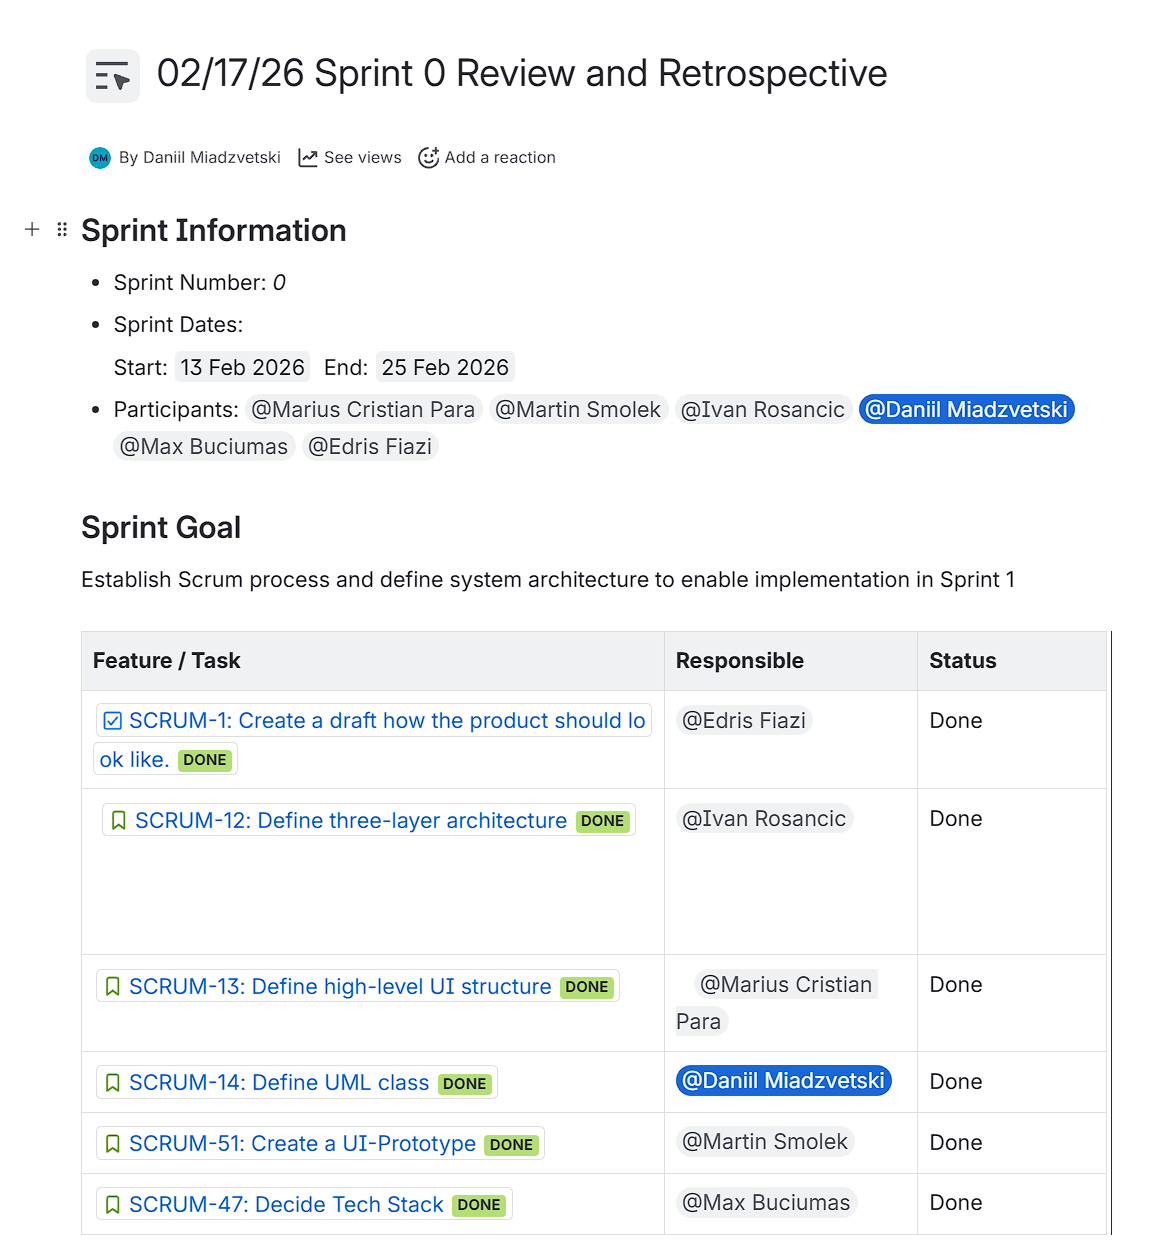
\includegraphics[width=\textwidth]{Images/PlanningReviewRetrospective/Sprint0PlanningAndReview.png}
    \caption{Sprint 0 Planning and Review evidence}
    \label{fig:sprint0-planning-review}
\end{figure}

\subsection*{Sprint Retrospective}

\begin{figure}[H]
    \centering
    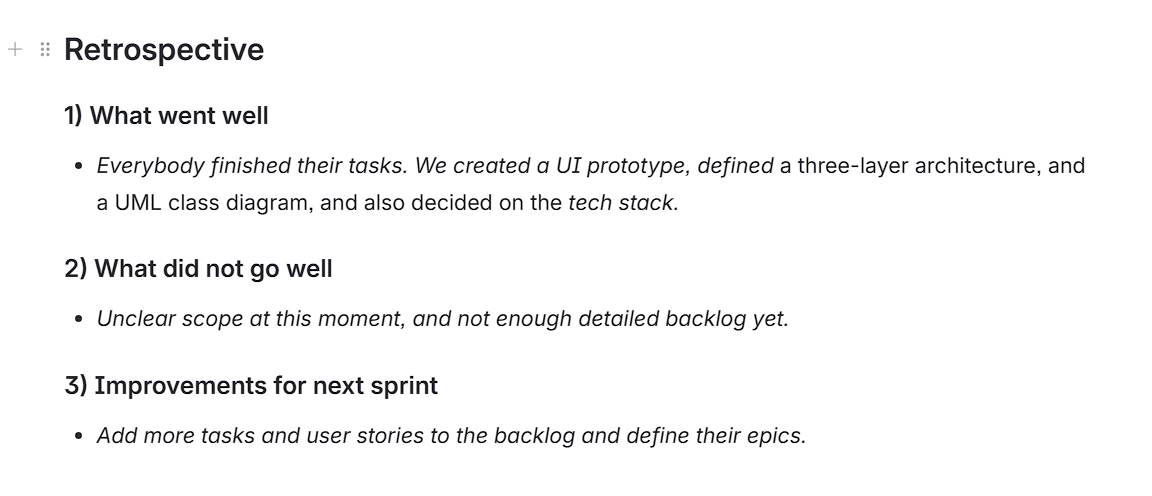
\includegraphics[width=0.9\textwidth]{Images/PlanningReviewRetrospective/Sprint0Retrospective.png}
    \caption{Sprint 0 Retrospective evidence}
    \label{fig:sprint0-retrospective}
\end{figure}

%========================================================
\section{Sprint 1}
\label{app:sprint1}

\subsection*{Sprint Planning}

\begin{figure}[H]
    \centering
    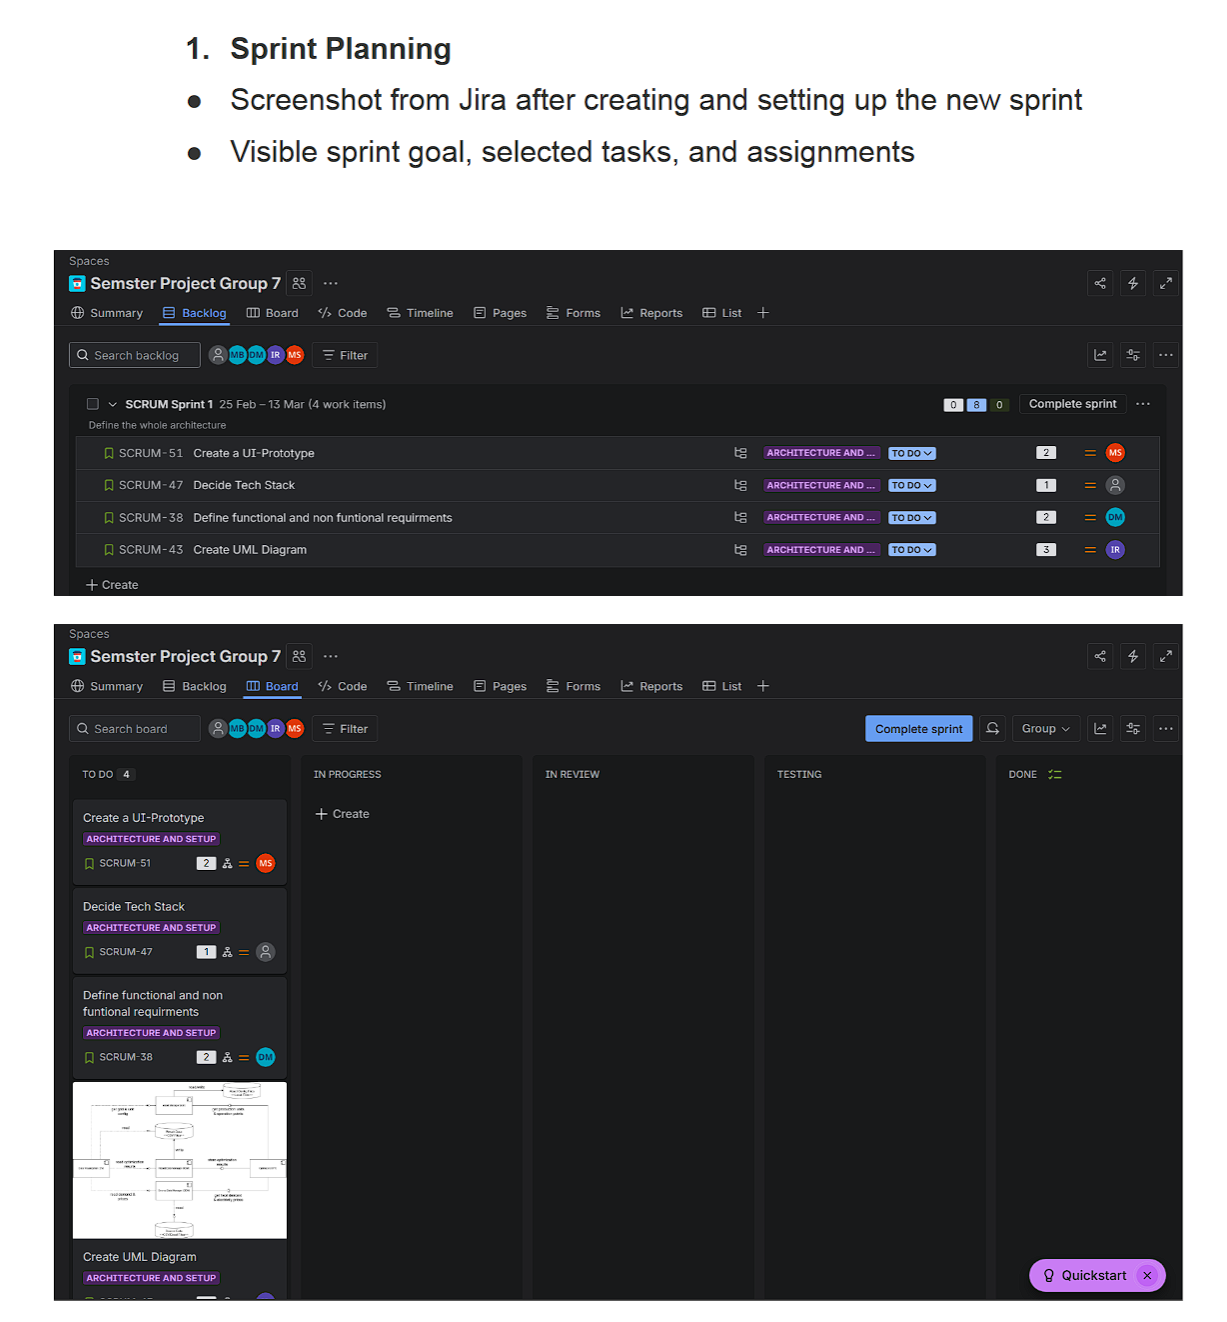
\includegraphics[width=\textwidth]{Images/PlanningReviewRetrospective/Sprint1Planning.png}
    \caption{Sprint 1 Planning evidence}
    \label{fig:sprint1-planning}
\end{figure}

\subsection*{Sprint Review}

\begin{figure}[H]
    \centering
    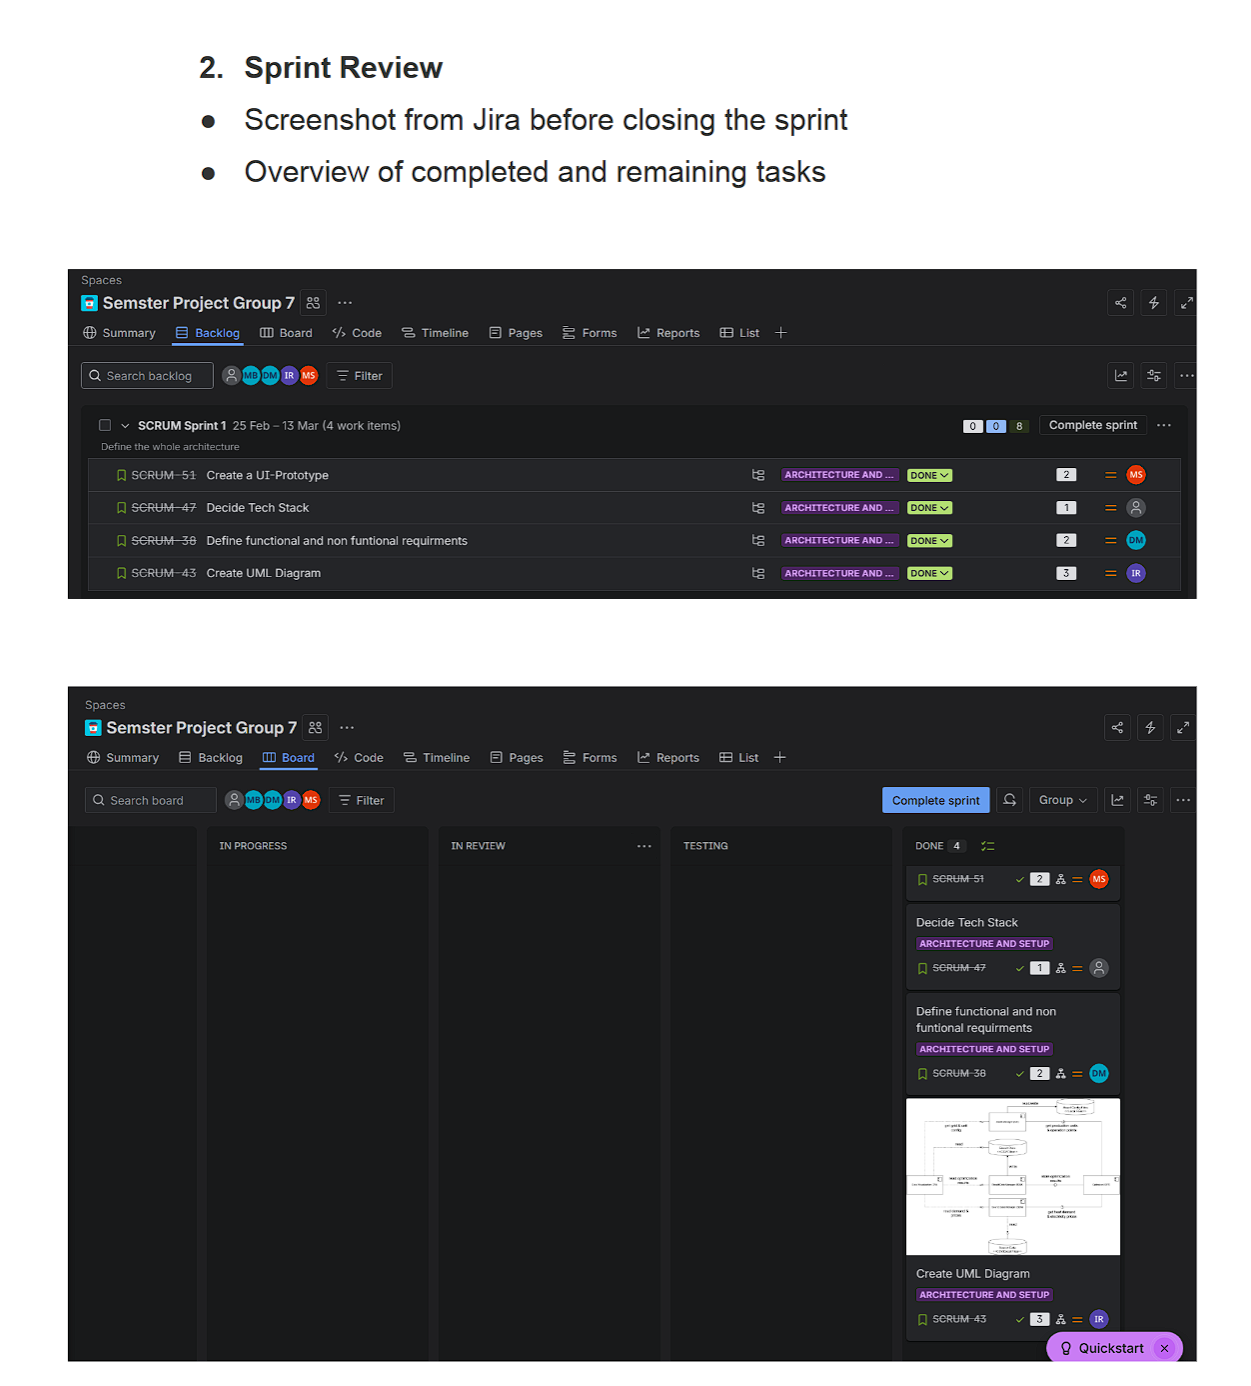
\includegraphics[width=\textwidth]{Images/PlanningReviewRetrospective/Sprint1Review.png}
    \caption{Sprint 1 Review evidence}
    \label{fig:sprint1-review}
\end{figure}

\begin{figure}[H]
    \centering
    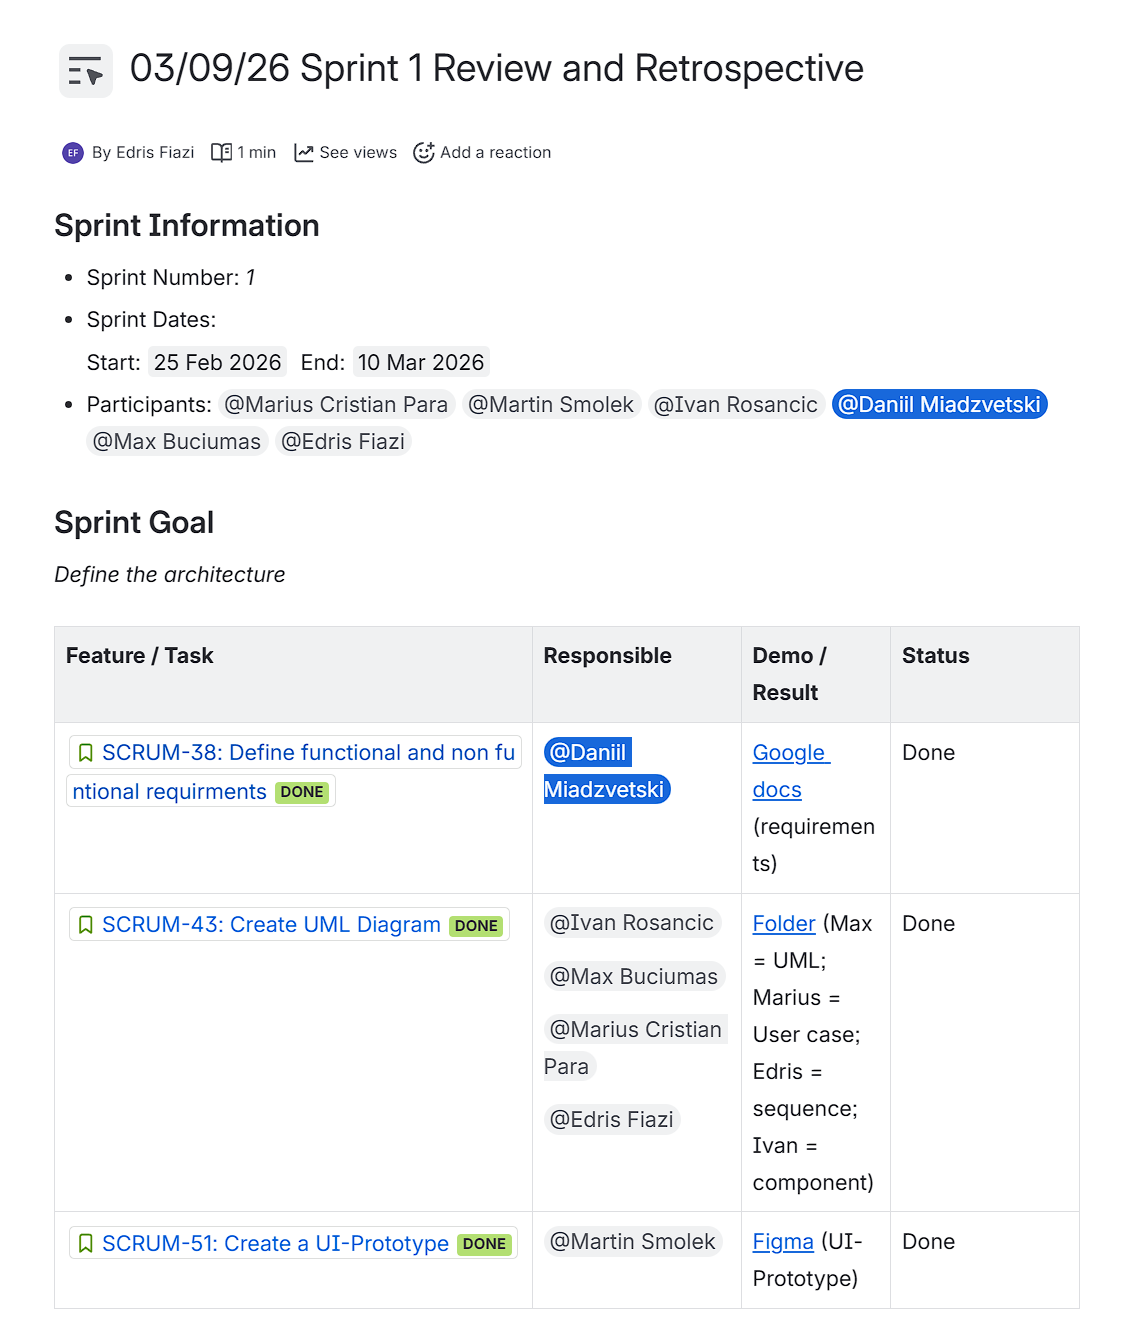
\includegraphics[width=\textwidth]{Images/PlanningReviewRetrospective/Sprint1Review2.png}
    \caption{Sprint 1 Review board overview}
    \label{fig:sprint1-review-board}
\end{figure}

\subsection*{Sprint Retrospective}

\begin{figure}[H]
    \centering
    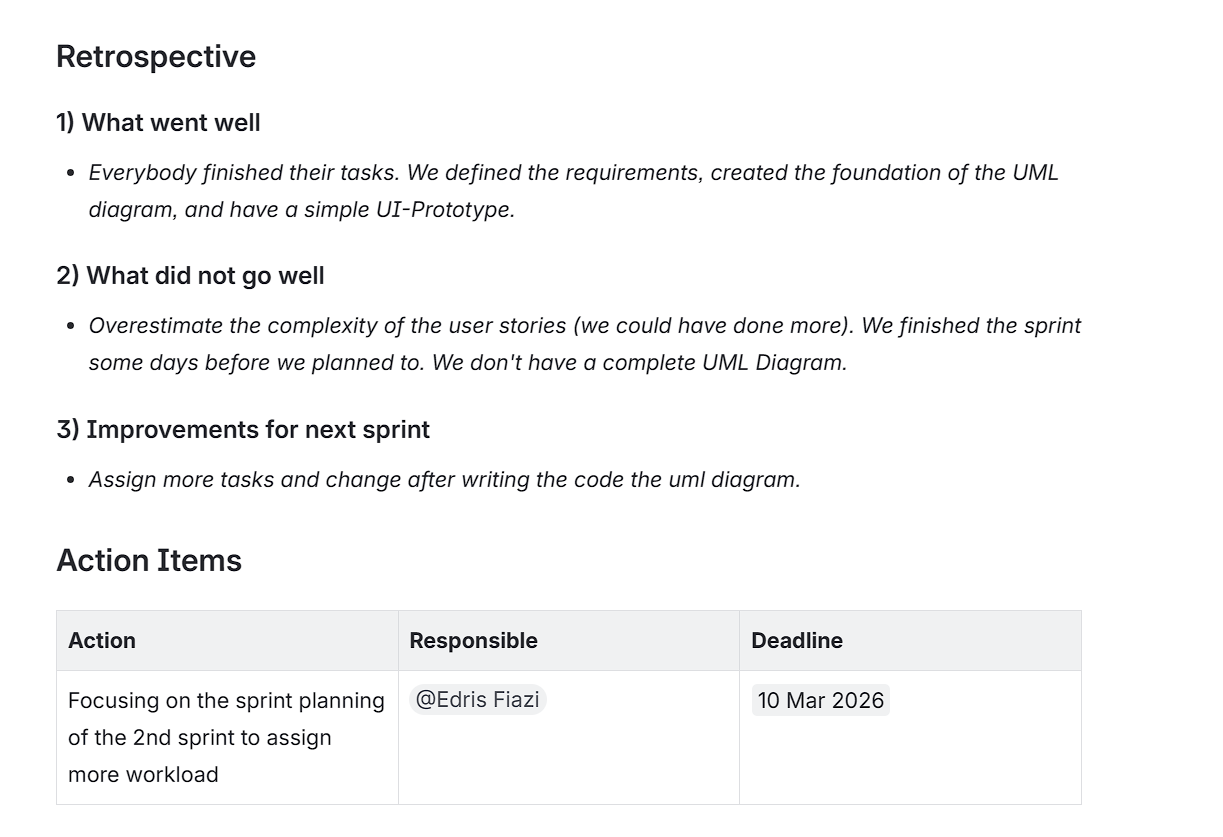
\includegraphics[width=\textwidth]{Images/PlanningReviewRetrospective/Sprint1Retrospective.png}
    \caption{Sprint 1 Retrospective evidence}
    \label{fig:sprint1-retrospective}
\end{figure}

%========================================================
\section{Sprint 2}
\label{app:sprint2}

\subsection*{Sprint Planning}

\begin{figure}[H]
    \centering
    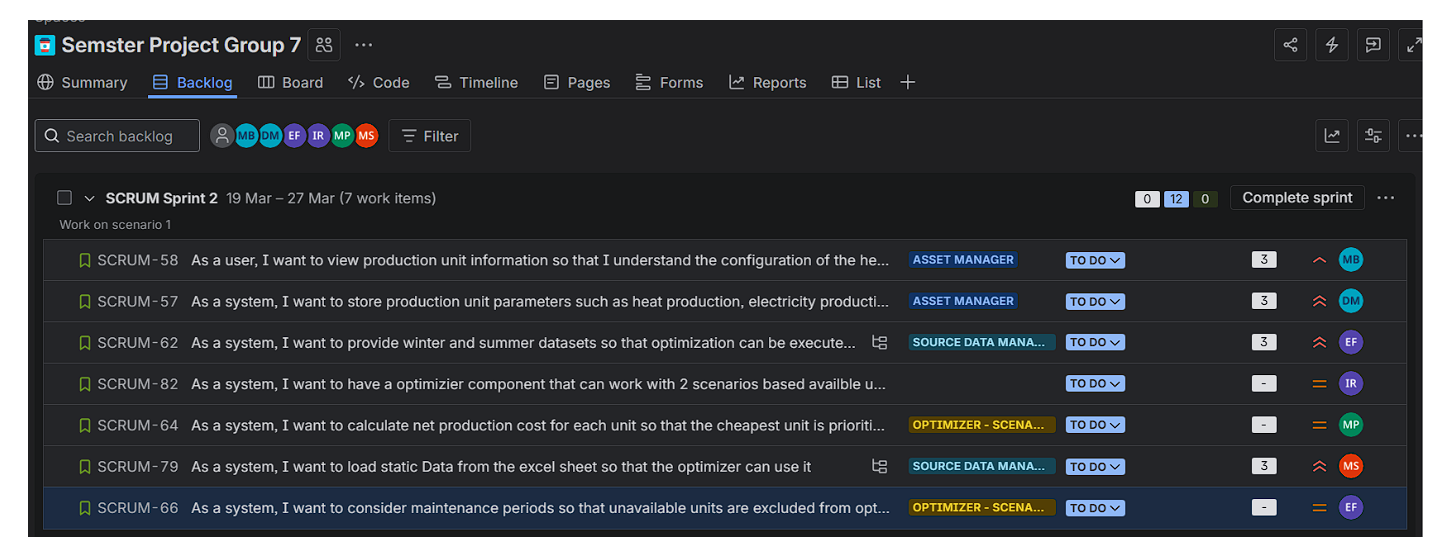
\includegraphics[width=\textwidth]{Images/PlanningReviewRetrospective/Sprint2Planning.png}
    \caption{Sprint 2 Planning evidence}
    \label{fig:sprint2-planning}
\end{figure}

\subsection*{Sprint Review}

\begin{figure}[H]
    \centering
    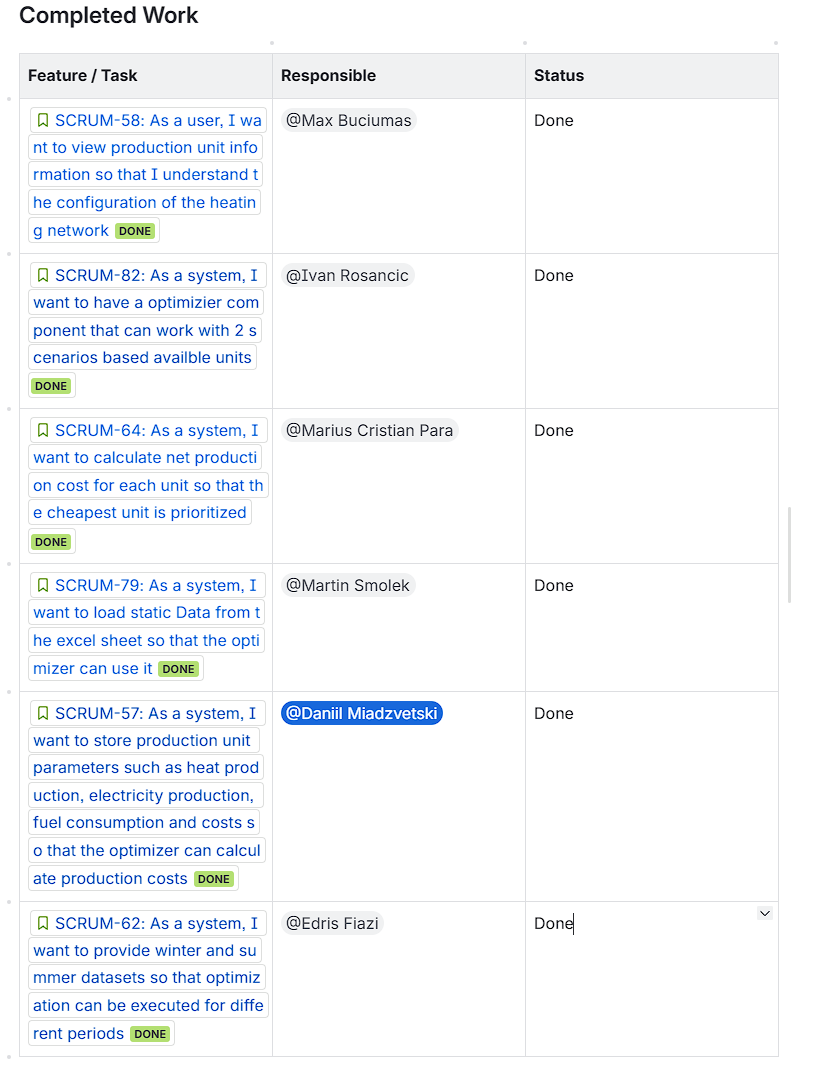
\includegraphics[width=\textwidth]{Images/PlanningReviewRetrospective/Sprint2Review.png}
    \caption{Sprint 2 Review evidence}
    \label{fig:sprint2-review}
\end{figure}

\subsection*{Sprint Retrospective}

\begin{figure}[H]
    \centering
    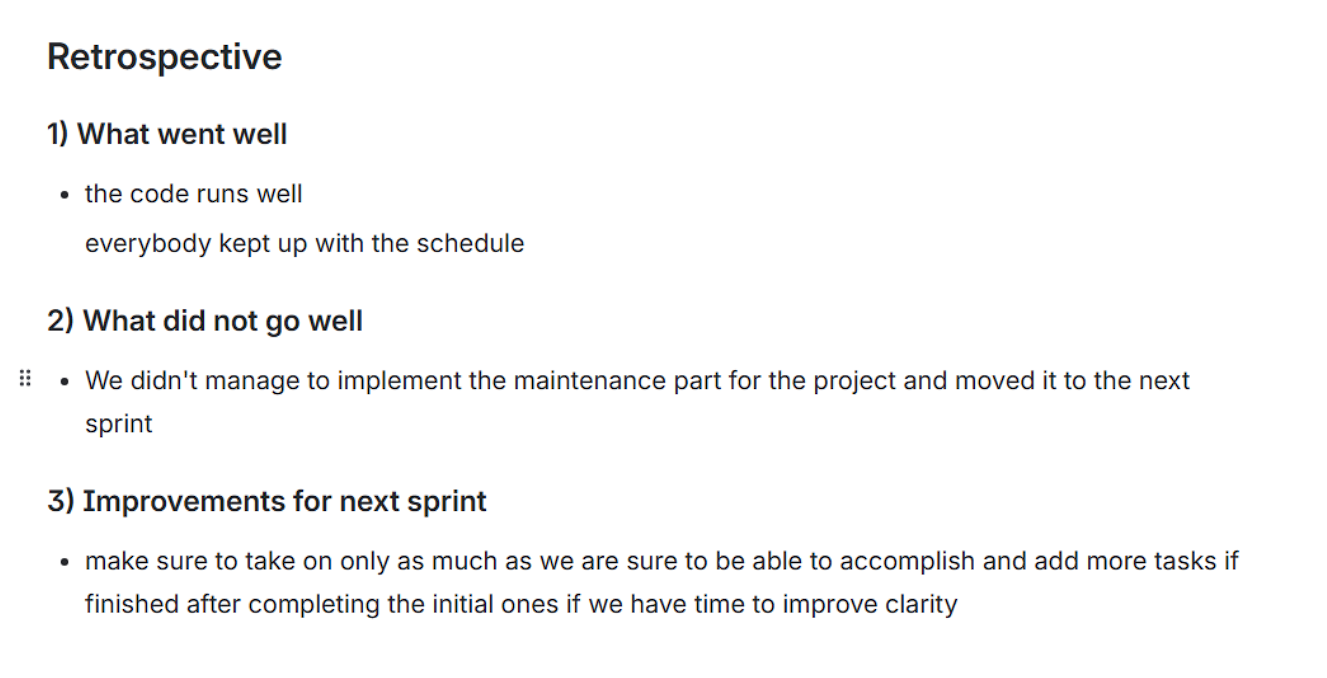
\includegraphics[width=\textwidth]{Images/PlanningReviewRetrospective/Sprint2Retrospective.png}
    \caption{Sprint 2 Retrospective evidence}
    \label{fig:sprint2-retrospective}
\end{figure}

%========================================================
\section{Sprint 3}
\label{app:sprint3}

\subsection*{Sprint Planning}

\begin{figure}[H]
    \centering
    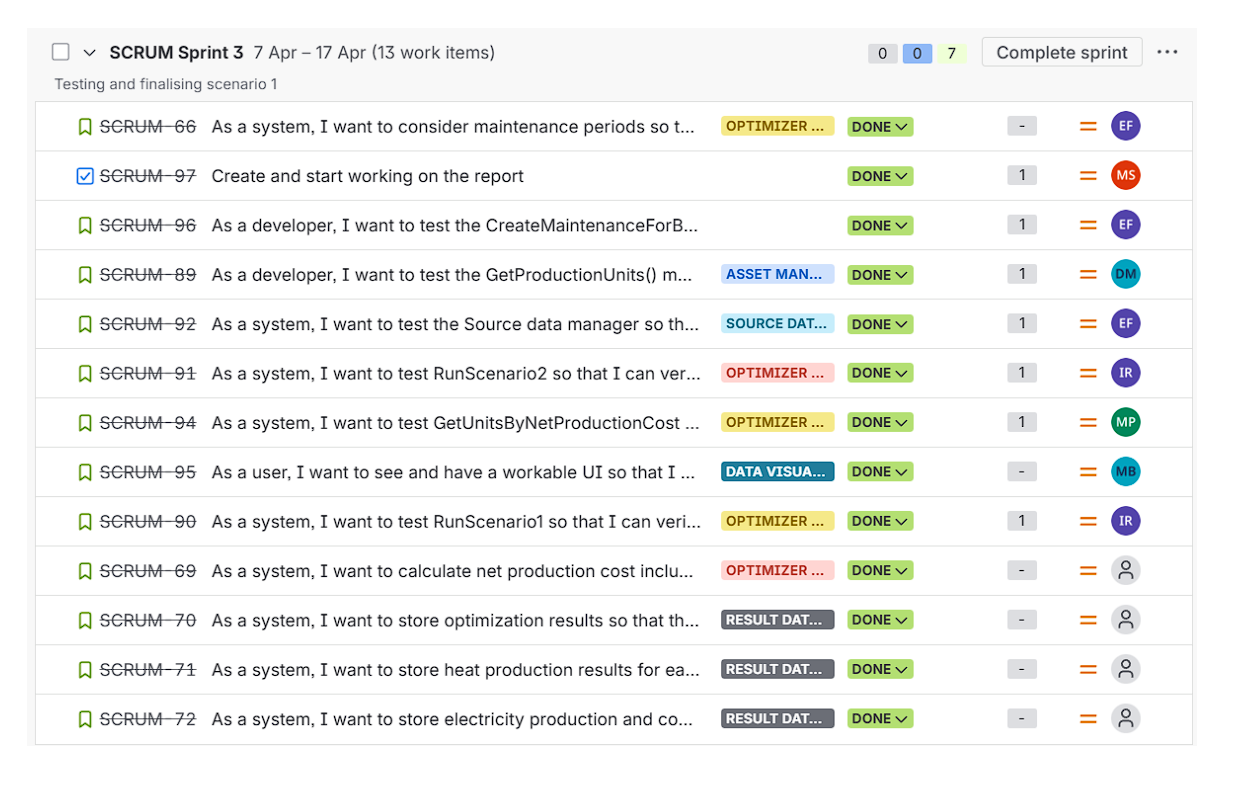
\includegraphics[width=\textwidth]{Images/PlanningReviewRetrospective/Sprint3Planning.png}
    \caption{Sprint 3 Planning evidence}
    \label{fig:sprint3-planning}
\end{figure}

\subsection*{Sprint Review}

\begin{figure}[H]
    \centering
    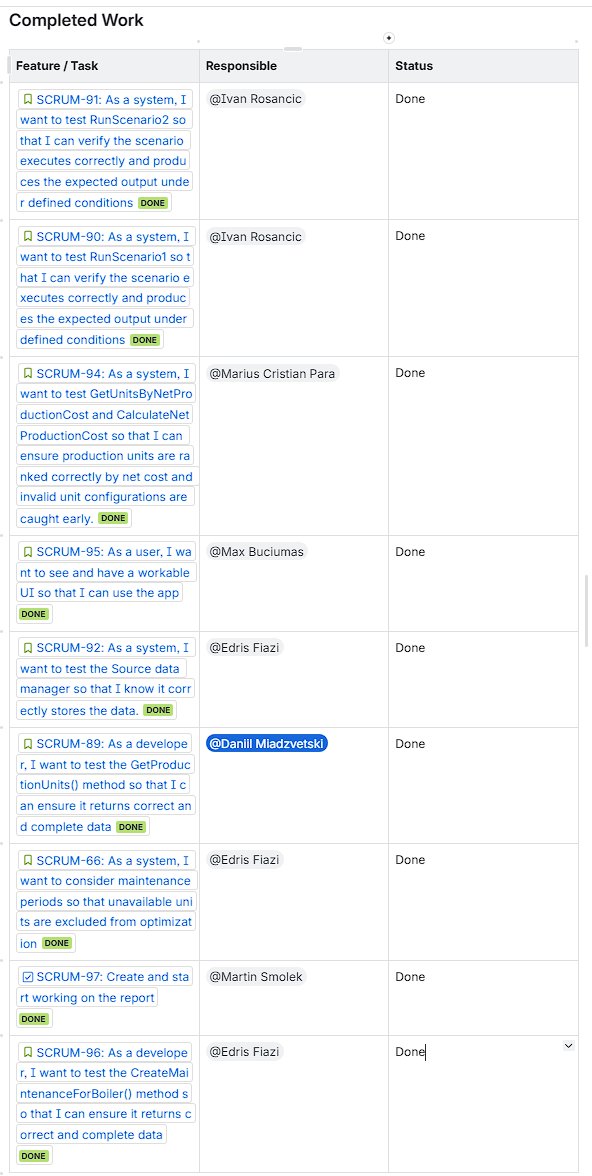
\includegraphics[width=\textwidth]{Images/PlanningReviewRetrospective/Sprint3PReview.png}
    \caption{Sprint 3 Review evidence}
    \label{fig:sprint3-review}
\end{figure}

\subsection*{Sprint Retrospective}

\begin{figure}[H]
    \centering
    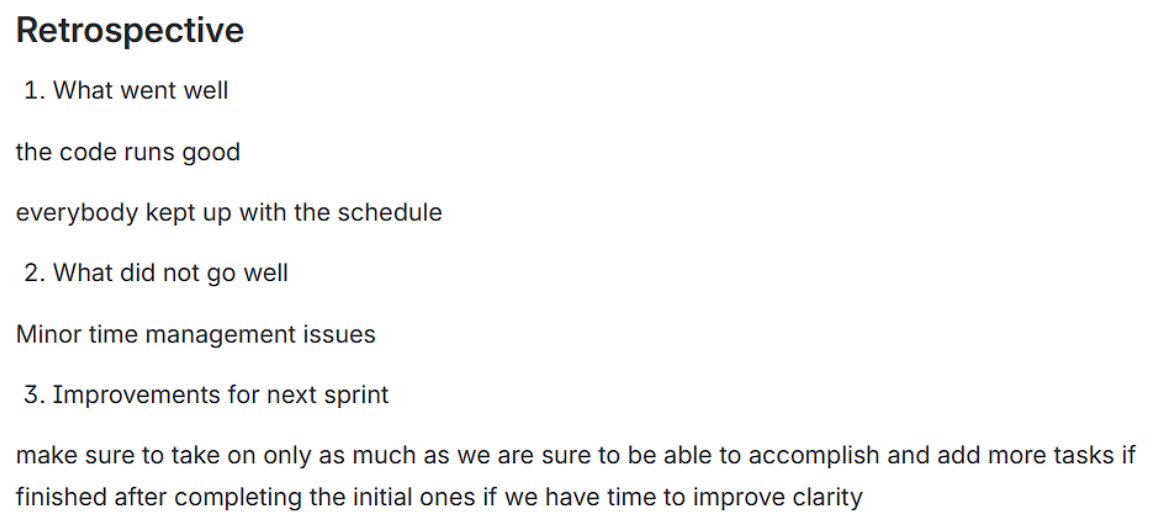
\includegraphics[width=\textwidth]{Images/PlanningReviewRetrospective/Sprint3Retrospective.png}
    \caption{Sprint 3 Retrospective evidence}
    \label{fig:sprint3-retrospective}
\end{figure}

%========================================================
\section{Sprint 4}
\label{app:sprint4}

\subsection*{Sprint Planning}

\begin{figure}[H]
    \centering
    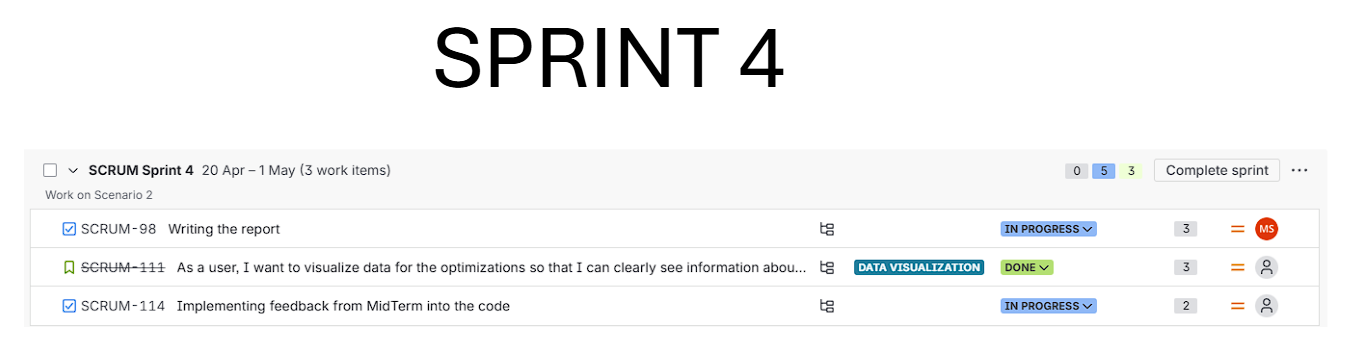
\includegraphics[width=\textwidth]{Images/PlanningReviewRetrospective/Sprint4Planning.png}
    \caption{Sprint 4 Planning evidence}
    \label{fig:sprint4-planning}
\end{figure}

\subsection*{Sprint Review}

\begin{figure}[H]
    \centering
    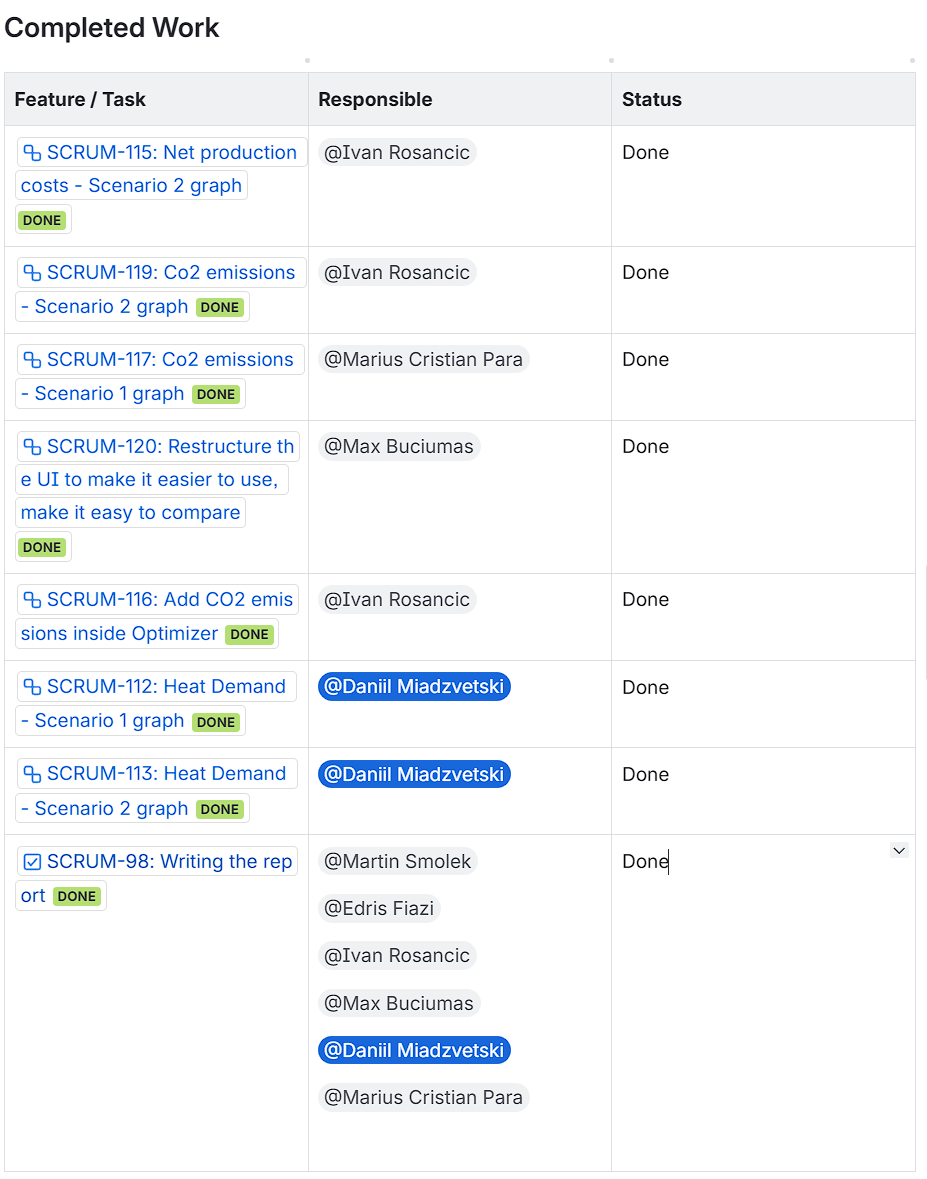
\includegraphics[width=\textwidth]{Images/PlanningReviewRetrospective/Sprint4Review.png}
    \caption{Sprint 4 Review evidence}
    \label{fig:sprint4-review}
\end{figure}

\subsection*{Sprint Retrospective}

\begin{figure}[H]
    \centering
    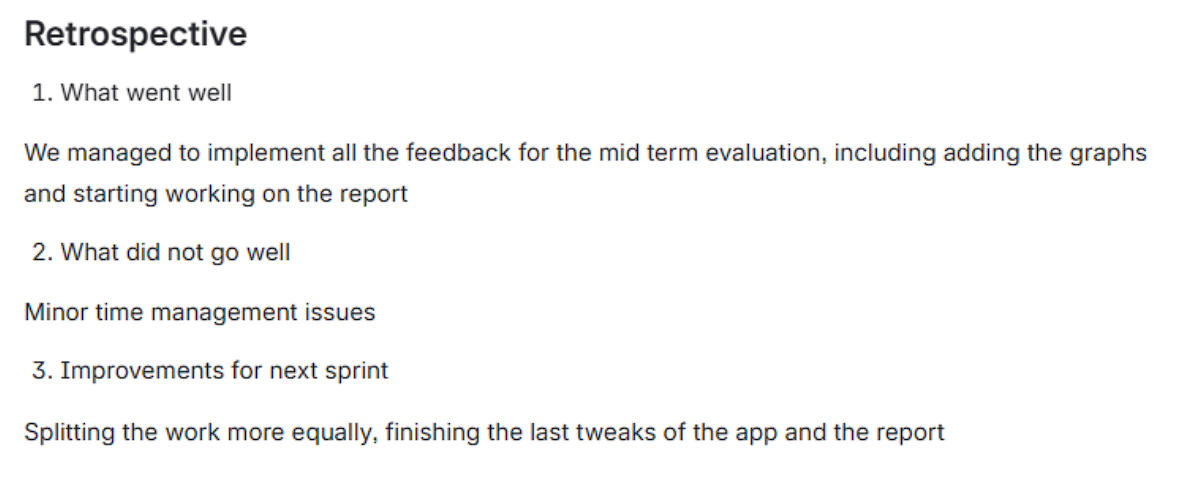
\includegraphics[width=\textwidth]{Images/PlanningReviewRetrospective/Sprint4Retrospective.png}
    \caption{Sprint 4 Retrospective evidence}
    \label{fig:sprint4-retrospective}
\end{figure}

%========================================================
\section{Sprint 5}
\label{app:sprint5}

\subsection*{Sprint Planning}

\begin{figure}[H]
    \centering
    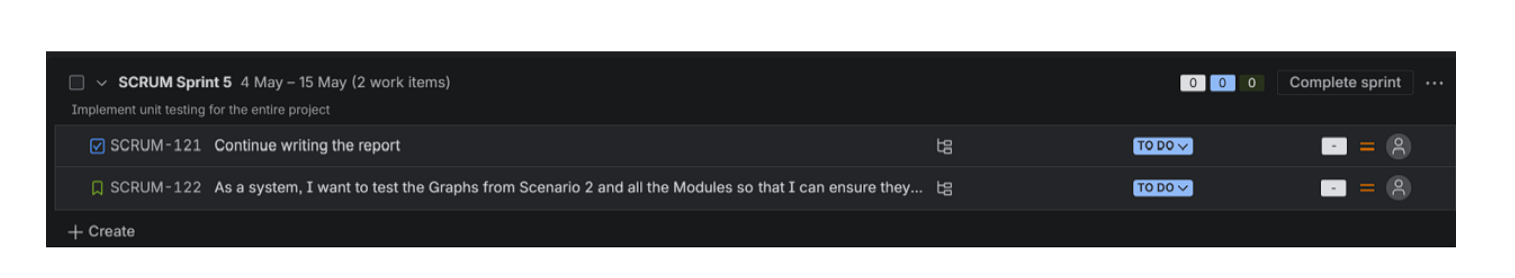
\includegraphics[width=\textwidth]{Images/PlanningReviewRetrospective/Sprint5Planning.png}
    \caption{Sprint 5 Planning evidence}
    \label{fig:sprint5-planning}
\end{figure}

\subsection*{Sprint Review}

\begin{figure}[H]
    \centering
    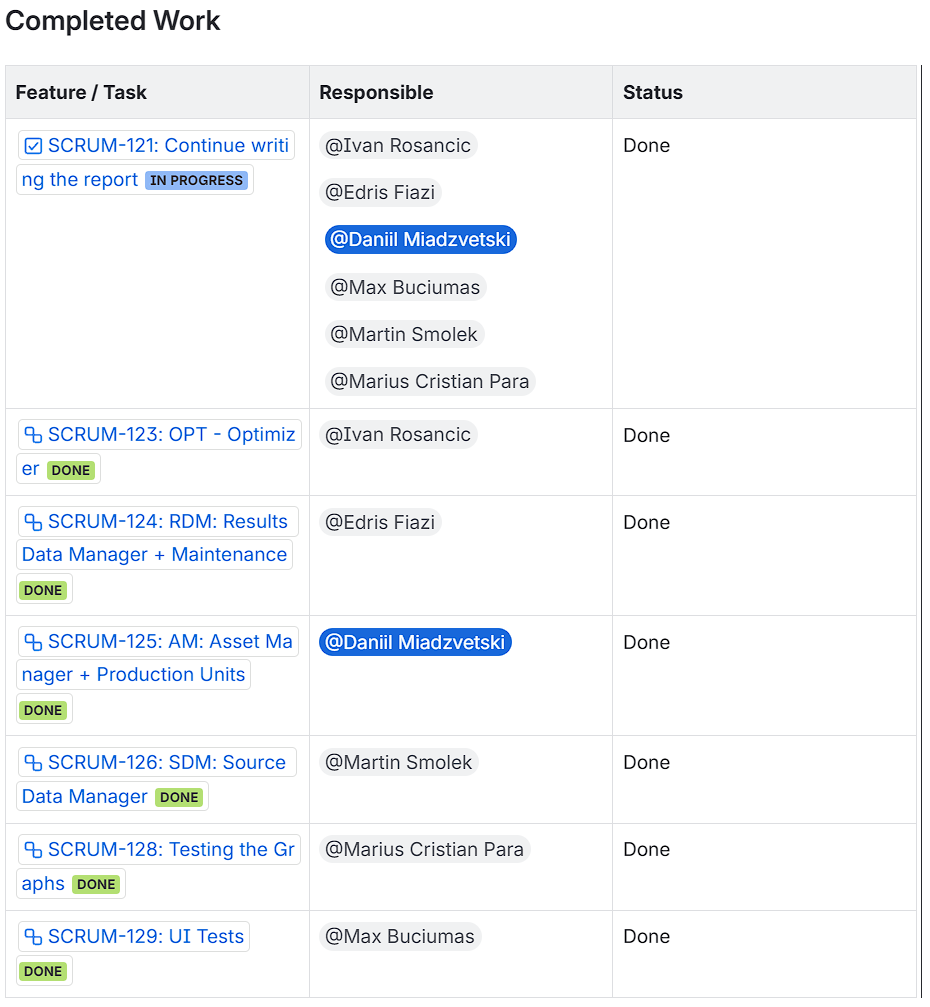
\includegraphics[width=\textwidth]{Images/PlanningReviewRetrospective/Sprint5Review.png}
    \caption{Sprint 5 Review evidence}
    \label{fig:sprint5-review}
\end{figure}

\subsection*{Sprint Retrospective}

\begin{figure}[H]
    \centering
    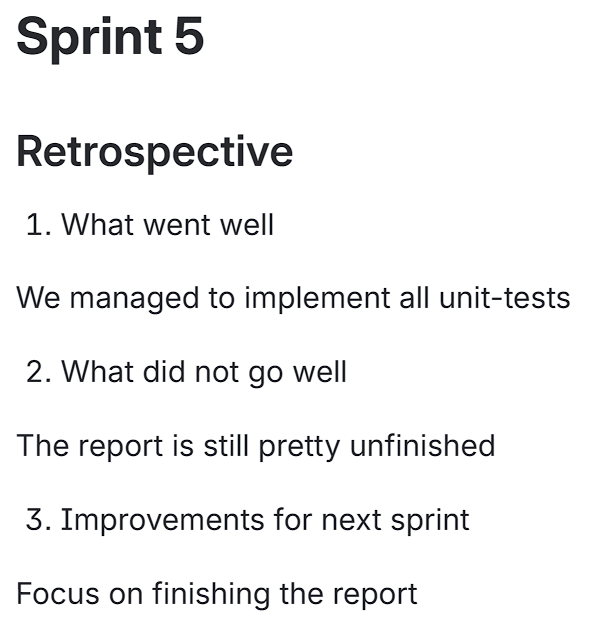
\includegraphics[width=0.9\textwidth]{Images/PlanningReviewRetrospective/Sprint5Retrospective.png}
    \caption{Sprint 5 Retrospective evidence}
    \label{fig:sprint5-retrospective}
\end{figure}


\end{document}